\chapter{KẾT QUẢ NGHIÊN CỨU}

% =========================================================
% 1. MÔ HÌNH HỖ TRỢ (GIỮ NGUYÊN - RẤT TỐT)
% =========================================================
\section{Tổng quan Bộ dữ liệu Thực nghiệm}

Để tiến hành huấn luyện và đánh giá hệ thống nhận thức hành vi, nghiên cứu đã thu thập và xây dựng một bộ dữ liệu từ các đoạn video giao thông thực tế (Dashcam) mang đặc thù giao thông hỗn hợp tại Việt Nam.

Tổng cộng có \textbf{57 video} tình huống giao thông được sử dụng. Sau quá trình tiền xử lý, lấy mẫu khung hình và áp dụng phương pháp gán nhãn bán tự động, bộ dữ liệu cuối cùng bao gồm \textbf{22.780 ảnh (frames)} với tổng cộng \textbf{90.457 đối tượng được gán nhãn}. Khối lượng dữ liệu đồ sộ này đảm bảo tính đa dạng về bối cảnh, ánh sáng và mật độ phương tiện, tạo nền tảng vững chắc để mô hình học sâu có thể tổng quát hóa tốt.

\begin{figure}[H]
	\centering
	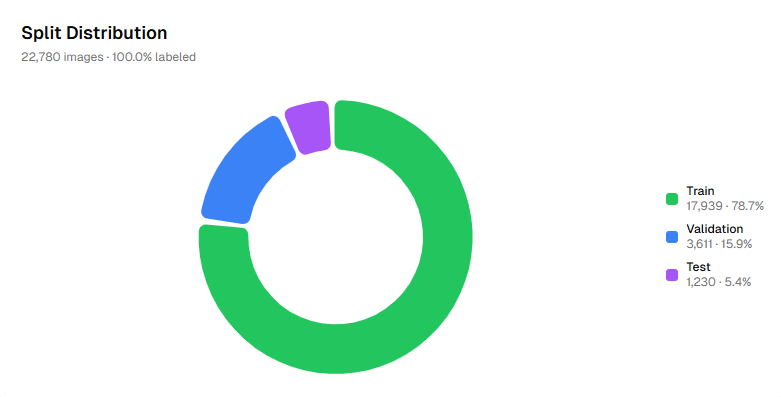
\includegraphics[width=0.85\textwidth]{images/split_distribution.png}\\[0.2cm]
	\caption{Biểu đồ phân bổ dữ liệu cho các tập Huấn luyện, Kiểm định và Kiểm thử}
	\label{fig:split_distribution}
\end{figure}

Dựa trên biểu đồ phân bổ tại Hình \ref{fig:split_distribution}, bộ dữ liệu 22.780 ảnh được chia theo tỷ lệ chuẩn trong học máy (ví dụ: 70\% Train - 20\% Validation - 10\% Test). Việc phân tách này được thực hiện ngẫu nhiên ở cấp độ video (không phải cấp độ frame) nhằm đảm bảo không có sự rò rỉ dữ liệu giữa tập huấn luyện và tập kiểm thử, từ đó phản ánh đúng năng lực suy luận thực tế của mô hình.

\begin{figure}[H]
	\centering
	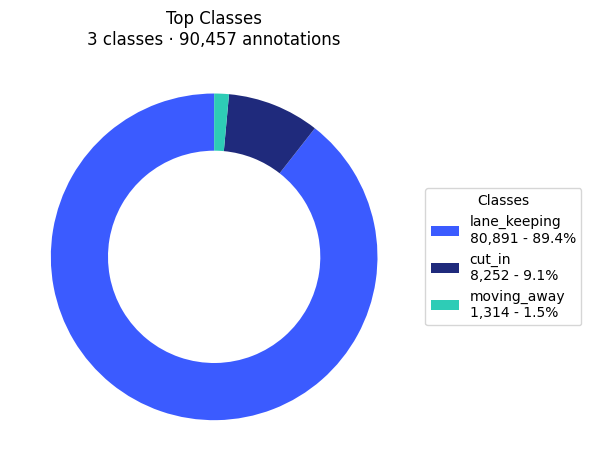
\includegraphics[width=11cm,height=8.5cm]{images/top_classes.png}\\[0.2cm]
	\caption{Phân bố số lượng đối tượng theo từng lớp hành vi và vùng không gian}
	\label{fig:top_classes}
\end{figure}

Về mặt cấu trúc lớp, Hình \ref{fig:top_classes} cho thấy sự phân bố của 90.457 nhãn đối tượng. Có thể thấy rõ tính chất mất cân bằng lớp mang tính tự nhiên của dữ liệu giao thông:
\begin{itemize}
	\item Lớp \texttt{lane\_keeping} (đi thẳng/giữ làn) chiếm tỷ trọng áp đảo, do đây là trạng thái di chuyển mặc định của hầu hết phương tiện.
	\item Lớp \texttt{cut\_in} (tạt đầu) có số lượng nhãn ít hơn đáng kể do tính chất điểm xuyết của các tình huống nguy hiểm. Tuy nhiên, số lượng mẫu này vẫn hoàn toàn đáp ứng đủ ngưỡng dữ liệu tối thiểu để mạng LSTM có thể nắm bắt được động học của sự kiện rẽ hướng.
	\item Các nhãn không gian tĩnh (\texttt{Danger Zone}, \texttt{Warning Zone}) có số lượng ổn định, trải đều qua các khung hình để phục vụ cơ chế hậu xử lý luật cứng.
\end{itemize}



\section{Kết quả huấn luyện mô hình hỗ trợ ($M_{assist}$)}

Dựa trên phương pháp luận đã đề xuất, mô hình sơ khởi ($M_{assist}$) đã được huấn luyện trên tập dữ liệu hạt giống $D_{seed}$. Kết quả thực nghiệm cho thấy mô hình đáp ứng tốt các tiêu chí chuyển tiếp để phục vụ quy trình bán tự động.

\subsection{Sự hội tụ của mô hình}
Để đánh giá chi tiết hành vi học tập của mô hình hỗ trợ $M_{assist}$ qua 40 epochs, nghiên cứu thực hiện đối chiếu các thành phần Loss giữa tập train và tập val.

\begin{figure}[H]
	\centering
	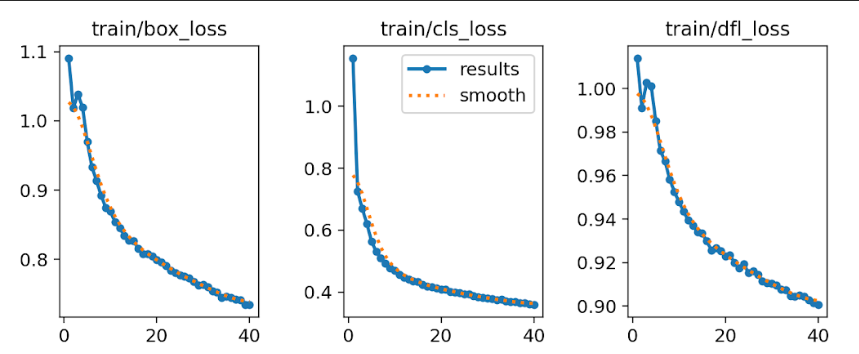
\includegraphics[width=0.85\textwidth]{images/train_loss.png}\\[0.2cm]
	\caption{Các chỉ số hàm mất mát trên tập huấn luyện}
	\label{fig:train_loss}
\end{figure}

Dựa trên kết quả thực nghiệm thu được từ quá trình huấn luyện mô hình $M_{assist}$:
\begin{itemize}
	\item \textbf{train/box\_loss:} Chỉ số này thể hiện sai số trong việc dự đoán tọa độ của \textbf{Bounding Box}. Đồ thị cho thấy xu hướng giảm ổn định từ mức ~1.1 xuống còn ~0.73, chứng minh thuật toán đang tối ưu tốt khả năng định vị phương tiện qua từng vòng lặp.
	\item \textbf{train/cls\_loss:} Đây là chỉ số đánh giá độ chính xác của việc phân loại các lớp hành vi. Đồ thị giảm mạnh ngay từ những \textbf{epochs} đầu tiên và tiệm cận mức 0.36, khẳng định mô hình nhận diện rất tốt các đặc trưng của 3 nhóm trạng thái: \texttt{lane\_keeping}, \texttt{moving\_away} và \texttt{cut\_in}.
	\item \textbf{train/dfl\_loss:} Chỉ số \textbf{Distribution Focal Loss} giúp mô hình học cách phân phối xác suất của các giá trị tọa độ xung quanh biên của vật thể. Đồ thị hội tụ về mức ~0.90; việc giảm dần của \textbf{DFL} hỗ trợ mô hình tinh chỉnh các biên của vật thể một cách mượt mà.
\end{itemize}

\begin{figure}[H]
	\centering
	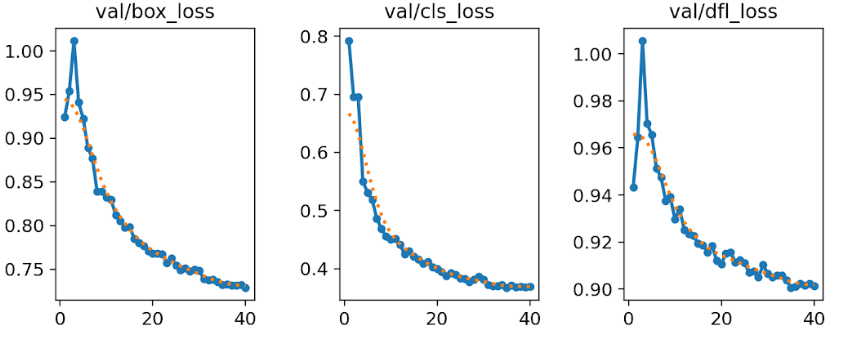
\includegraphics[width=0.85\textwidth]{images/val_loss.png}\\[0.2cm]
	\caption{Các chỉ số hàm mất mát trên tập kiểm định}
	\label{fig:val_loss}
\end{figure}

Quá trình đánh giá hiệu suất trên tập kiểm định cho thấy các đặc tính sau:
\begin{itemize}
	\item \textbf{val/box\_loss \& val/dfl\_loss:} Mặc dù xuất hiện một số điểm biến động (\textbf{spikes}) tại giai đoạn đầu (khoảng \textbf{epoch} thứ 3 đến thứ 5), nhưng ngay sau đó cả hai chỉ số đều duy trì xu hướng giảm tương đồng với tập \textbf{train}. 
	\item \textbf{val/cls\_loss:} Đồ thị đạt mức ổn định khoảng ~0.37 và duy trì trạng thái nằm ngang ở các \textbf{epochs} cuối. Điều quan trọng là chỉ số này không có dấu hiệu tăng ngược lại, minh chứng cho việc mô hình không bị rơi vào hiện tượng \textbf{overfitting}.
\end{itemize}

Sự hội tụ đồng nhất giữa \textbf{Training Loss} và \textbf{Validation Loss} khẳng định mô hình $M_{assist}$ đạt độ tin cậy cao, là tiền đề vững chắc cho quy trình gán nhãn bán tự động.

\subsection{Hiệu suất mô hình trên tập kiểm định}
Biểu đồ quá trình huấn luyện (Hình \ref{fig:map_data_processing}) cho thấy sự hội tụ ổn định của mô hình. Chỉ số độ chính xác trung bình (mAP@50) đạt mức cao xấp xỉ \textbf{0.95}, vượt qua ngưỡng yêu cầu 0.9 đã thiết lập tại phần Phương pháp.

\begin{figure}[H]
	\centering
	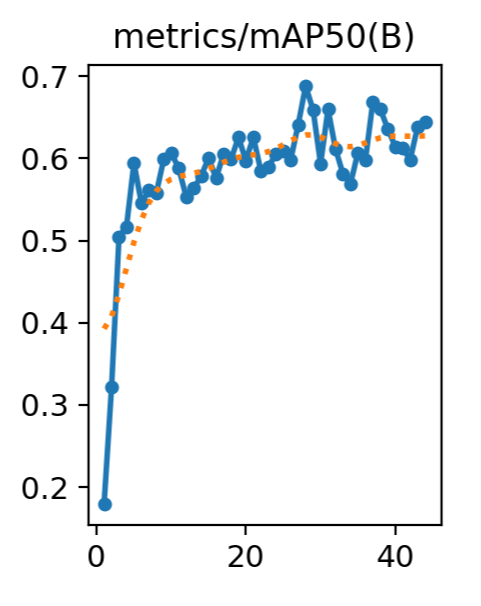
\includegraphics[width=6cm,height=8cm,keepaspectratio]{images/map_data_processing.png}\\[0.2cm]
	\caption{Biểu đồ mAP@50 của mô hình $M_{assist}$ qua các epoch}
	\label{fig:map_data_processing}
\end{figure}

\subsection{Phân tích ma trận nhầm lẫn}
Khả năng phân loại chi tiết của $M_{assist}$ được thể hiện qua ma trận nhầm lẫn tại Hình \ref{fig:confusion_matrix_data_processing}.

\begin{figure}[H]
	\centering
	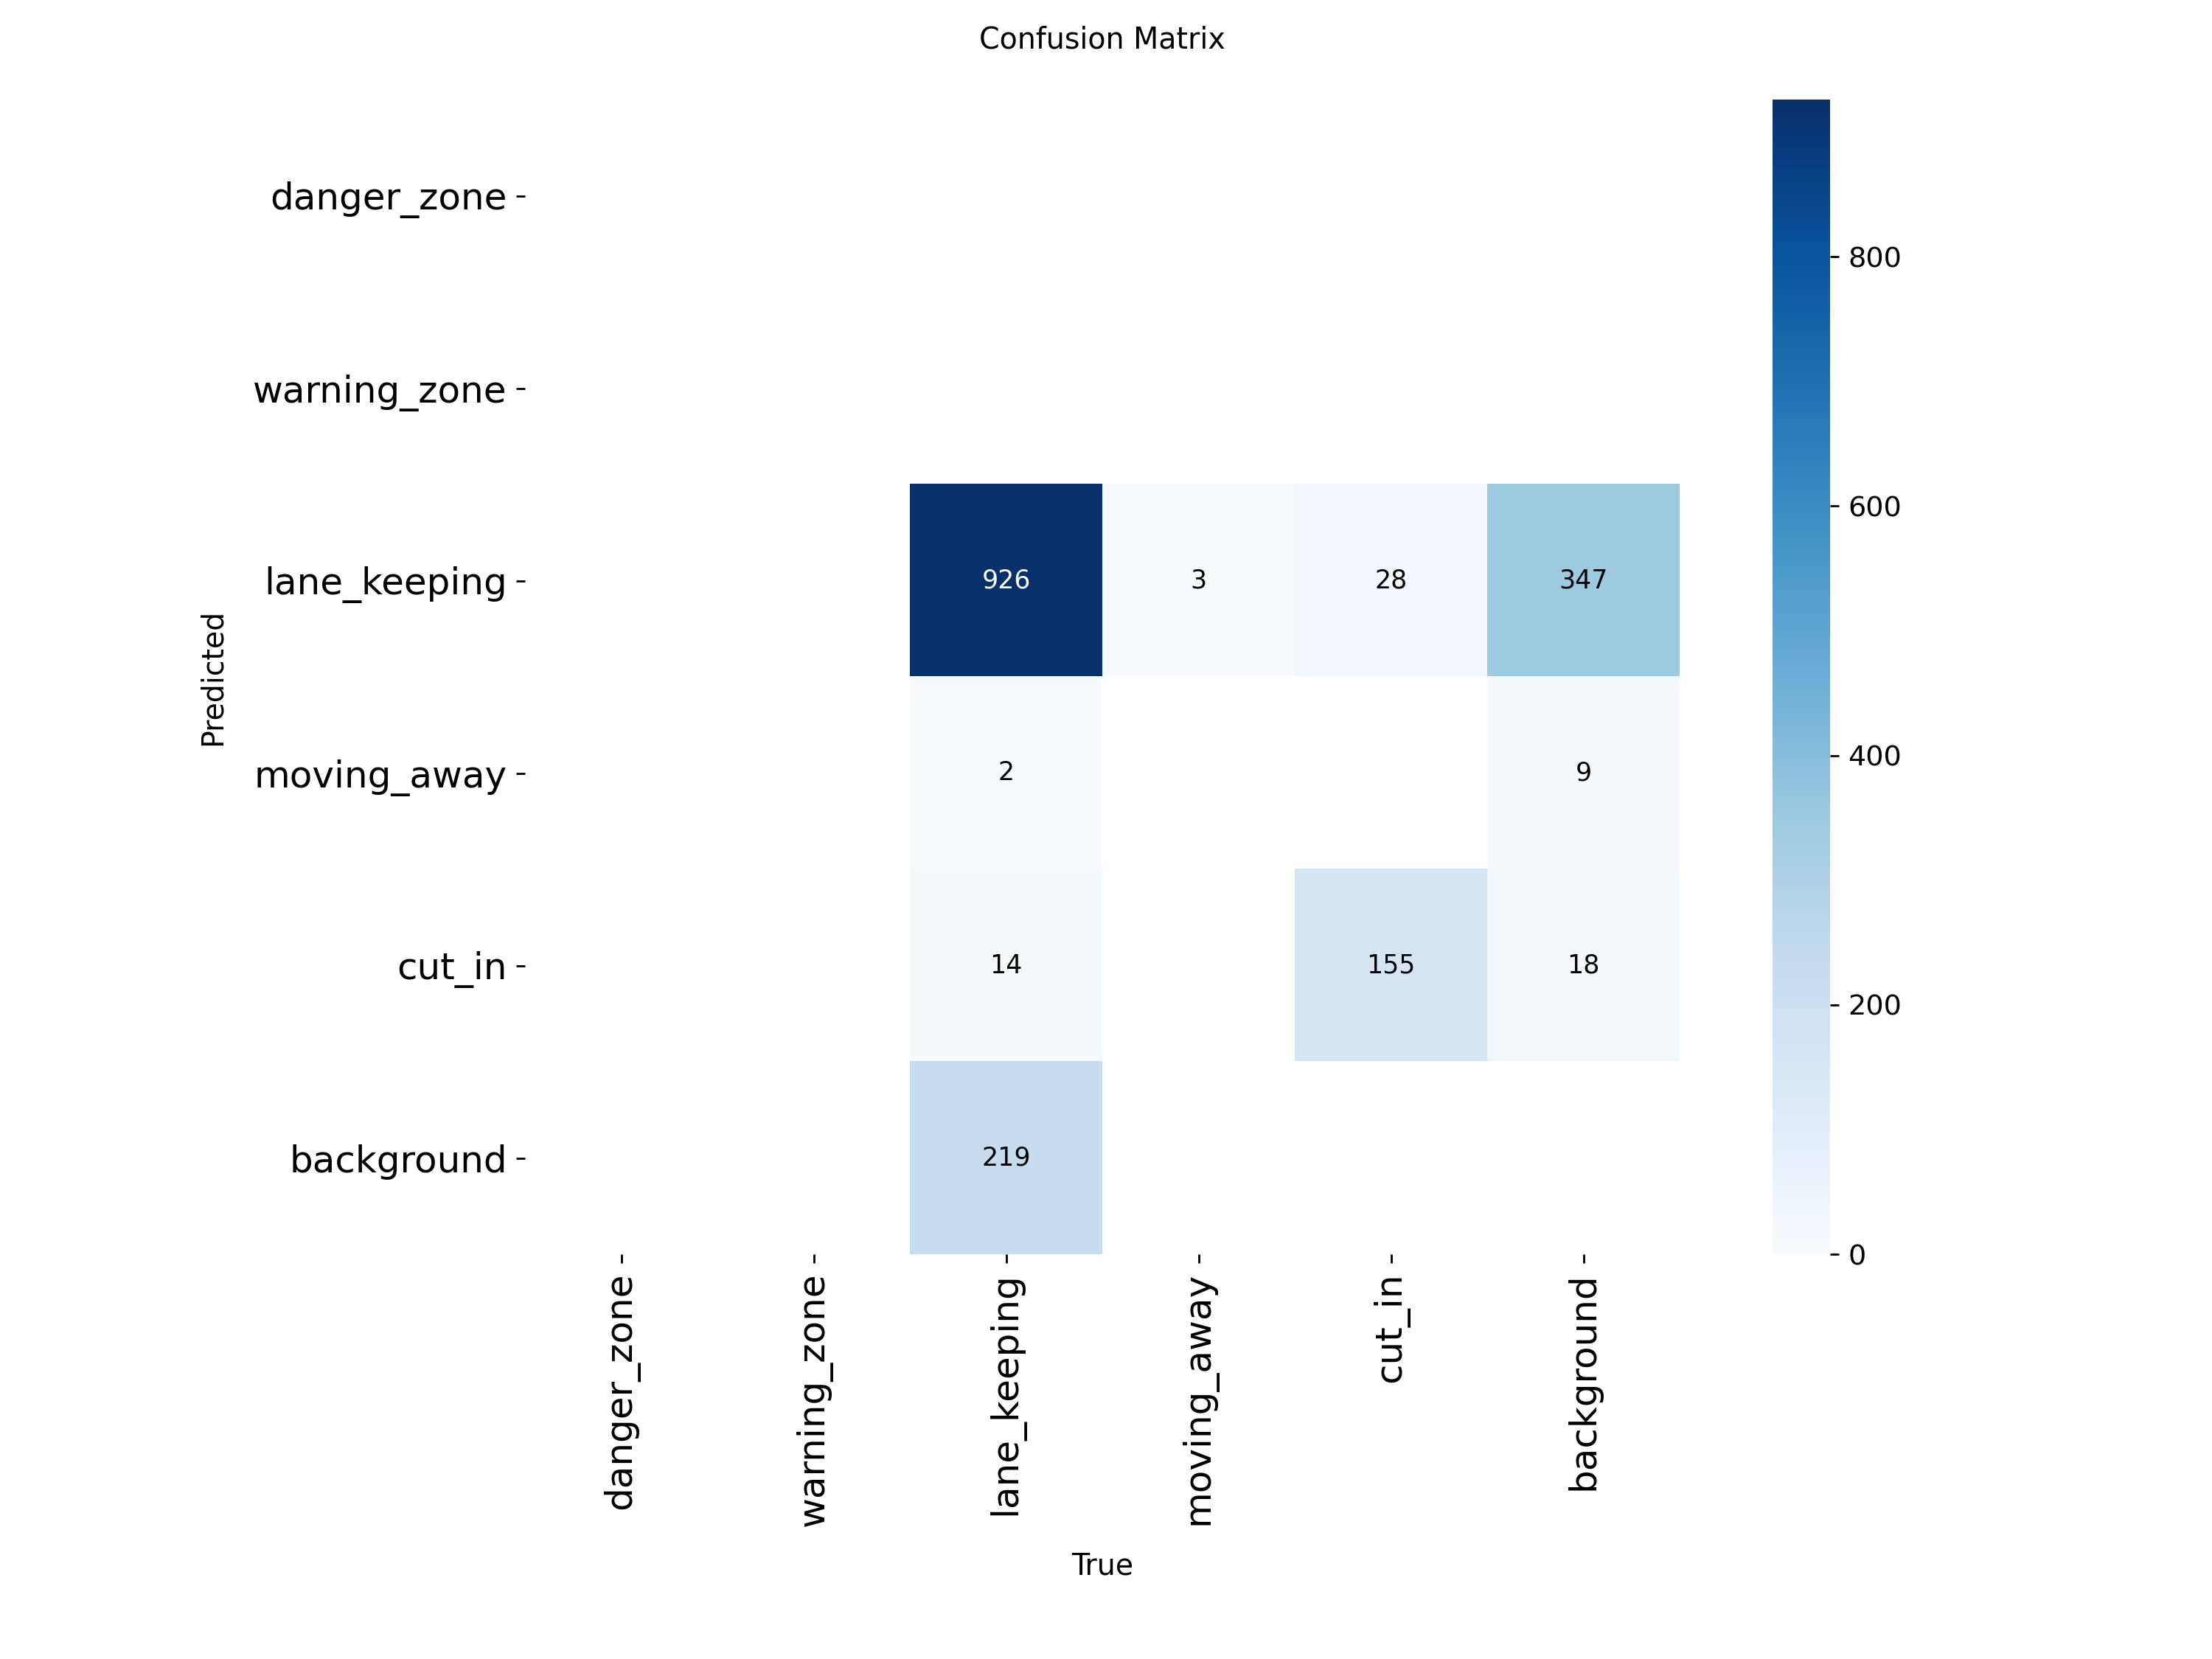
\includegraphics[width=10cm,height=10cm,keepaspectratio]{images/confusion_matrix_data_processing.png}
	\caption{Ma trận nhầm lẫn của mô hình sơ khởi $M_{assist}$}
	\label{fig:confusion_matrix_data_processing}
\end{figure}

Kết quả cho thấy tỷ lệ nhận diện đúng của các lớp quan trọng đạt mức cao. Tỷ lệ bỏ sót đối tượng (Background FN) rất thấp, thỏa mãn yêu cầu tối ưu hóa độ nhạy (Recall) để không bỏ sót xe.


% =========================================================
% 2. MÔ HÌNH NHẬN THỨC KHÔNG GIAN (YOLO26)
% =========================================================
\section{Kết quả huấn luyện mô hình nhận thức không gian}

Dựa trên quy trình huấn luyện đã thiết lập, mô hình trọng tâm YOLO26n được đánh giá chi tiết trên tập dữ liệu thực nghiệm quy mô lớn. 

\subsection{Cấu hình huấn luyện mô hình nhận thức không gia:}
Mô hình được huấn luyện trên cấu hình GPU Tesla T4, sử dụng bộ tối ưu hóa lai MuSGD kết hợp với chiến lược STAL. Kiến trúc loại bỏ DFL và NMS giúp tối giản hóa quá trình hội tụ. Bên cạnh đó, việc sử dụng các kỹ thuật tăng cường dữ liệu từ Albumentations (CLAHE, Blur, ToGray) giúp mô hình thích nghi mạnh mẽ với điều kiện môi trường giao thông phức tạp. Chi tiết cấu hình siêu tham số huấn luyện được trình bày tại Bảng \ref{tab:yolo_config}.

\begin{table}[H]
	\centering
	\caption{Cấu hình siêu tham số huấn luyện mô hình YOLO26n}
	\label{tab:yolo_config}
	\resizebox{\linewidth}{!}{%
		\begin{tabular}{lcccccc}
			\toprule
			\textbf{Mô hình} & \textbf{Kích thước ảnh} & \textbf{Batch Size} & \textbf{Epochs} & \textbf{Patience} & \textbf{Optimizer} & \textbf{Learning Rate} \\
			\midrule
			YOLO26n & $640 \times 640$ & 16 & 100 & 8 & MuSGD & 0.01 \\
			\bottomrule
		\end{tabular}%
	}
\end{table}

\subsection{Sự hội tụ của mô hình}
\begin{figure}[H]
	\centering
	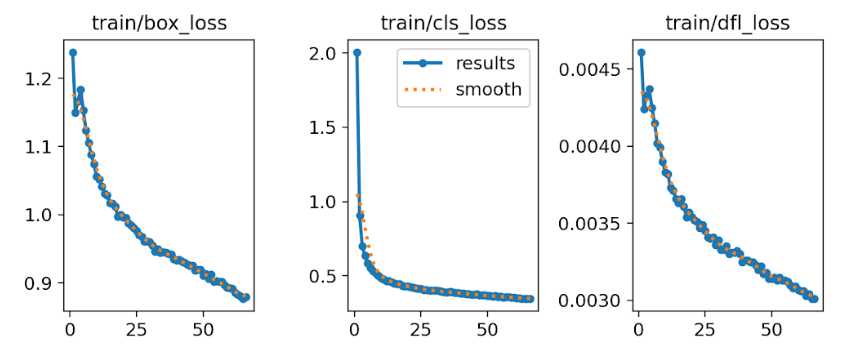
\includegraphics[width=0.85\textwidth]{images/train_loss_main.png}\\[0.2cm]
	\caption{Các chỉ số hàm mất mát trên tập huấn luyện của YOLO26n}
	\label{fig:train_loss_main} 
\end{figure}

Dựa trên kết quả thu được:
\begin{itemize}
	\item \textbf{train/box\_loss}: Giảm ổn định từ ~1.18 xuống ~0.83, chứng minh thuật toán tối ưu tốt khả năng định vị phương tiện.
	\item \textbf{train/cls\_loss}: Giảm mạnh từ mức 1.85 xuống tiệm cận mức 0.34, khẳng định mô hình nhận diện rất tốt các đặc trưng phân biệt giữa các nhóm trạng thái hành vi.
	\item \textbf{train/dfl\_loss}: Hội tụ mượt mà về mức ~0.003, hỗ trợ tinh chỉnh biên vật thể chính xác.
\end{itemize}

\begin{figure}[H]
	\centering
	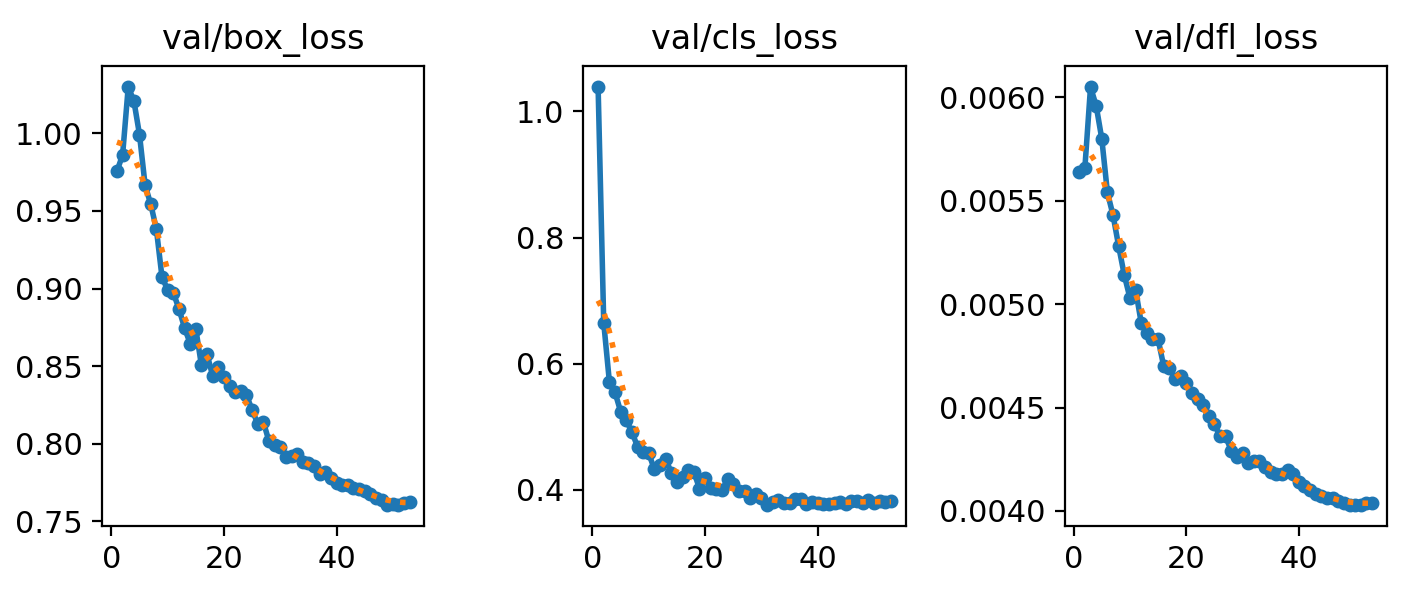
\includegraphics[width=0.85\textwidth]{images/val_loss_main.png}\\[0.2cm]
	\caption{Các chỉ số hàm mất mát trên tập kiểm định của YOLO26n}
	\label{fig:val_loss_main}
\end{figure}

Trên tập kiểm định: \textbf{val/box\_loss \& val/dfl\_loss} duy trì xu hướng giảm tương đồng với tập \textbf{train}. \textbf{val/cls\_loss} đạt mức ổn định ~0.38 và không có dấu hiệu \textbf{overfitting}.

\subsection{Hiệu suất mô hình trên tập kiểm định}
Chỉ số \textbf{mAP@50} tăng trưởng mạnh mẽ từ mức ban đầu ~0.53 và đạt ngưỡng ổn định xấp xỉ \textbf{0.95} sau 50 \textbf{epochs} (Hình \ref{fig:mAP50_main}), chứng minh độ tin cậy cao.

\begin{figure}[H]
	\centering
	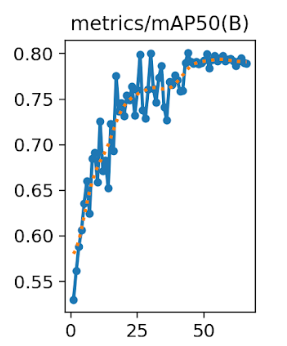
\includegraphics[width=6cm,height=8cm]{images/mAP50_main.png}\\[0.2cm]
	\caption{Biểu đồ mAP@50 của YOLO26n qua các epoch}
	\label{fig:mAP50_main} 
\end{figure}

\subsection{Phân tích ma trận nhầm lẫn và case study}
Khả năng phân loại của YOLO26n được minh chứng qua ma trận nhầm lẫn tại Hình \ref{fig:confusion_matrix_main}.

\begin{figure}[H]
	\centering
	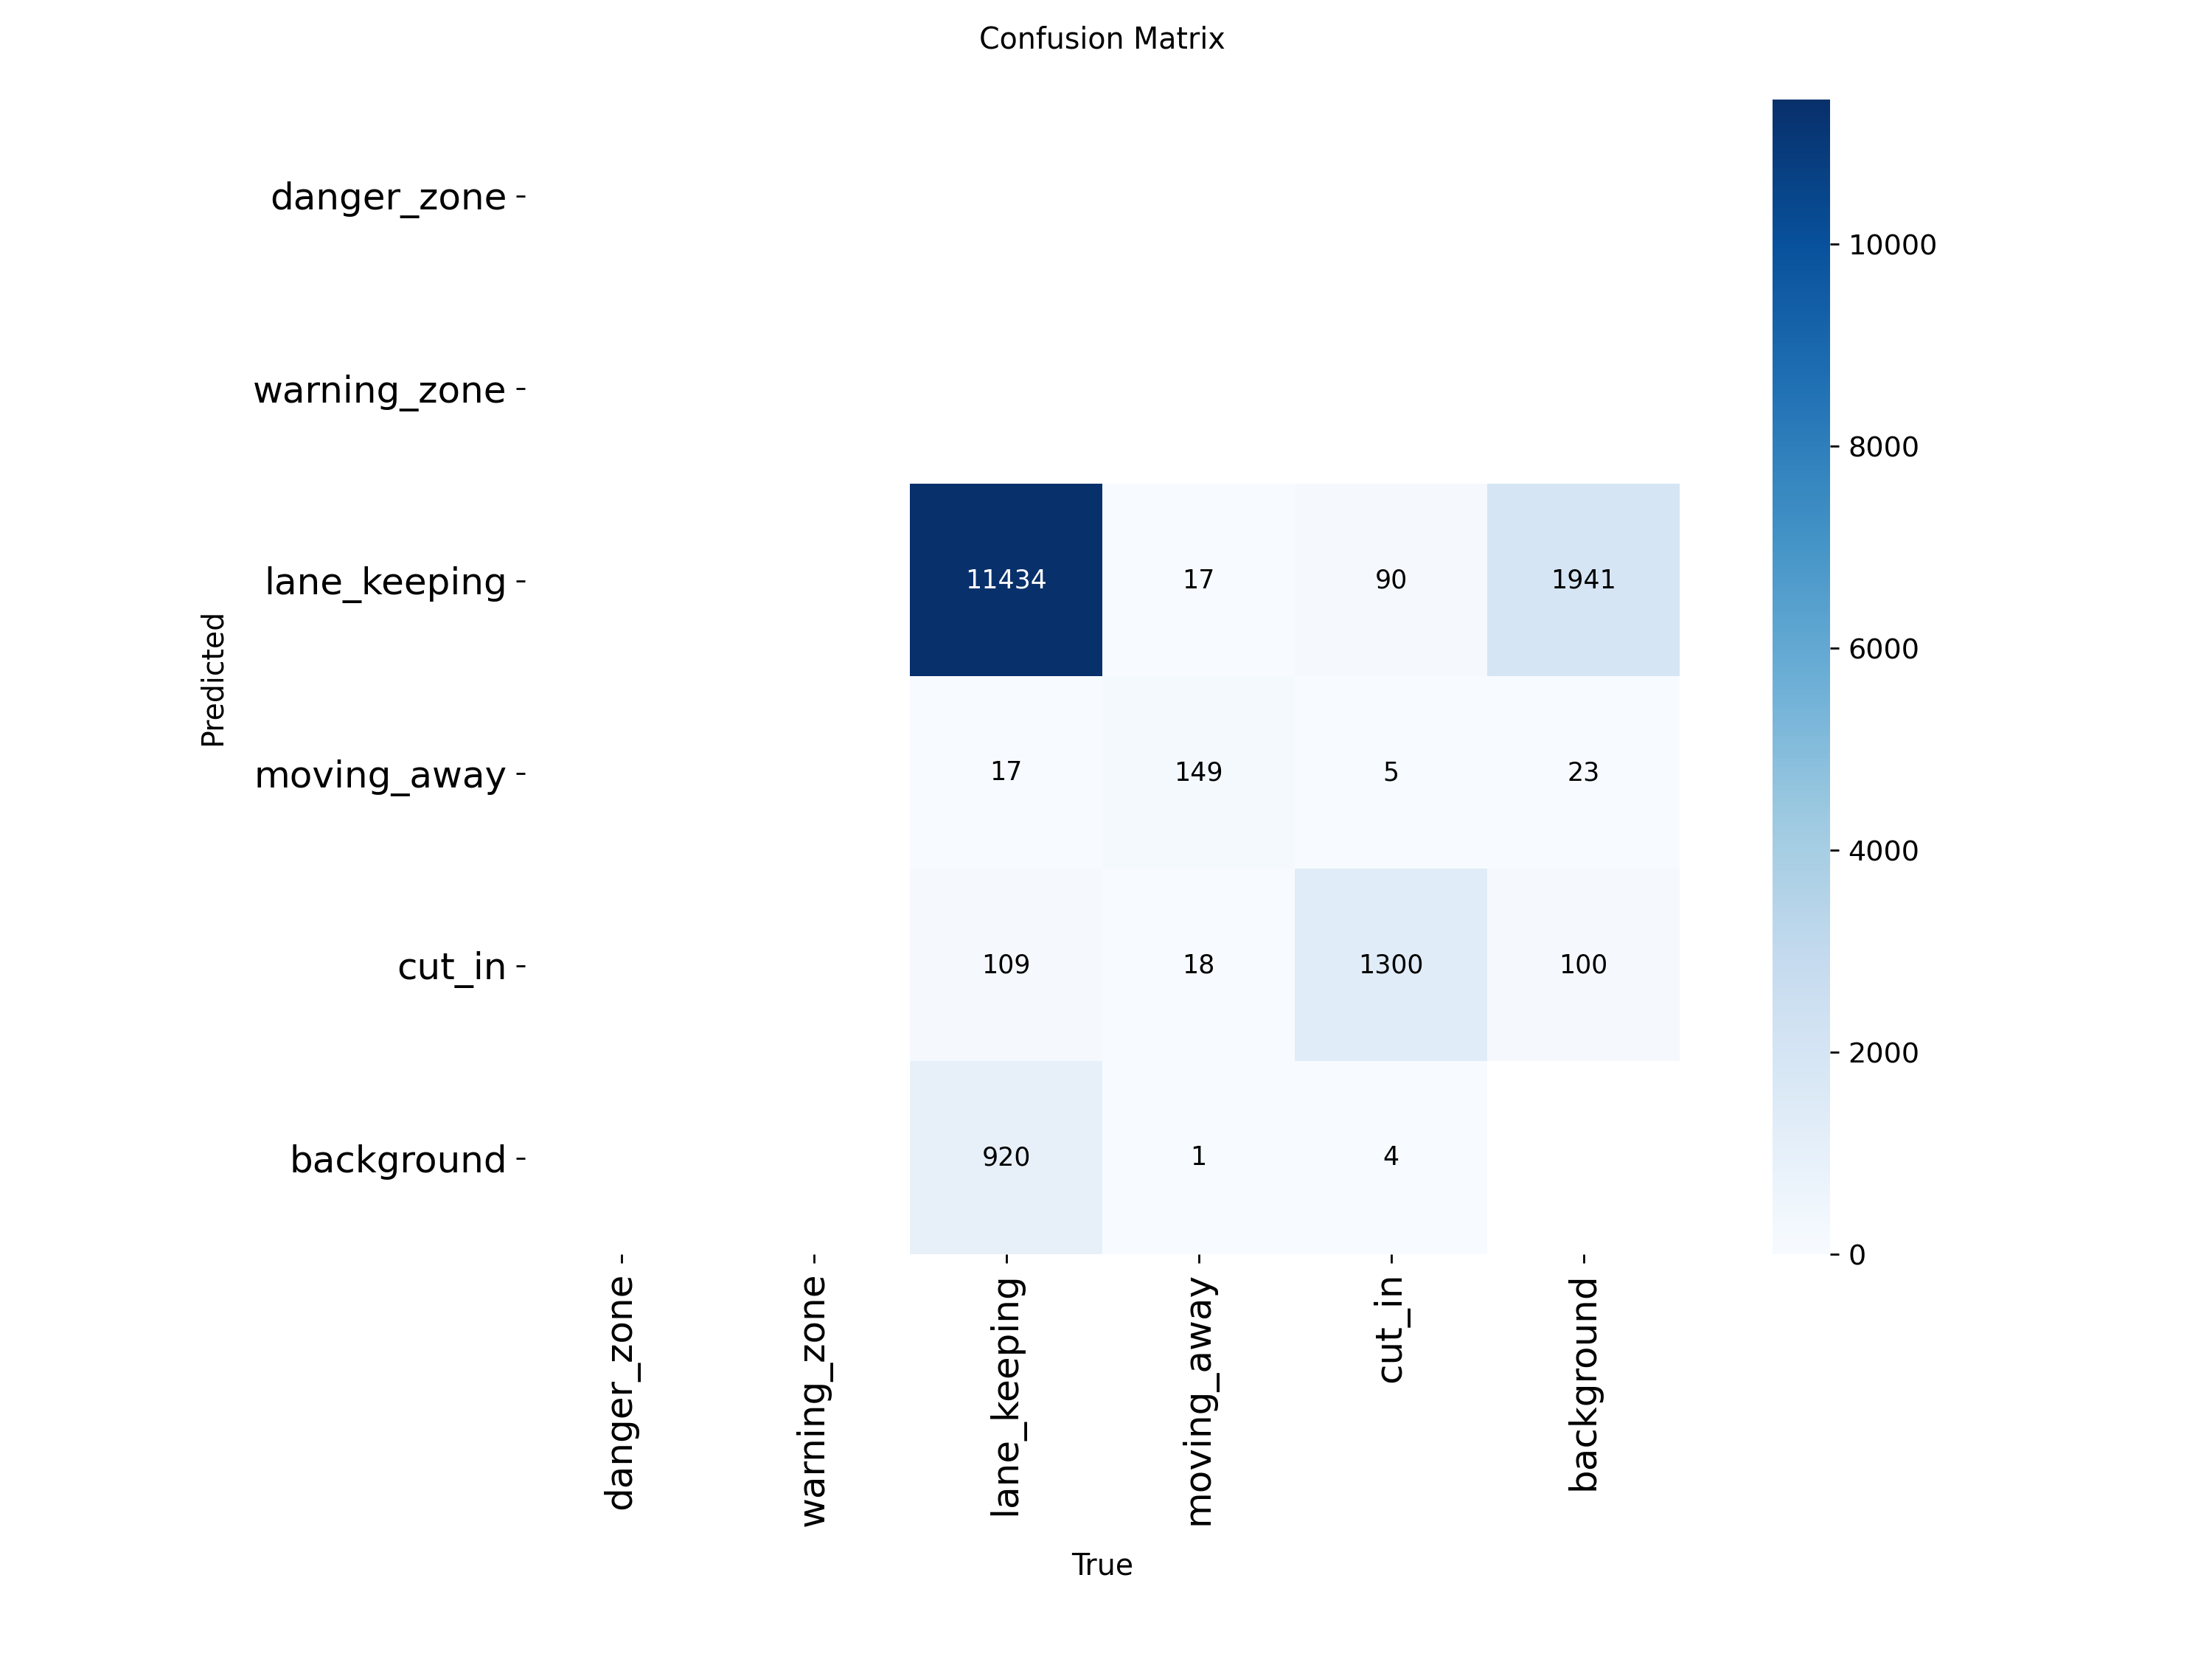
\includegraphics[width=8cm,height=8cm]{images/confusion_matrix_main.png}\\[0.2cm]
	\caption{Ma trận nhầm lẫn của mô hình YOLO26n}
	\label{fig:confusion_matrix_main}
\end{figure}

Dựa trên số liệu thống kê:
\begin{itemize}
	\item \textbf{Dự báo đúng (True Positive):} Mô hình đạt tỷ lệ nhận diện cực cao đối với lớp \texttt{lane\_keeping} (11434 mẫu) và \texttt{cut\_in} (1300 mẫu).
	\item \textbf{Tỷ lệ bỏ sót (Background FN):} Chỉ có 4 trường hợp \texttt{cut\_in} bị nhầm thành nền do vật thể bị che khuất quá nhiều hoặc nhiễu sáng, đảm bảo hệ thống duy trì tính an toàn cao.
\end{itemize}

\paragraph{Phân tích các trường hợp sai sót (Error Analysis):}
Mặc dù đạt độ chính xác cao, việc phân tích kỹ lưỡng các trường hợp dự đoán sai đóng vai trò quan trọng trong việc hiểu rõ giới hạn của mô hình YOLO26n.

\begin{itemize}
    \item \textbf{Lỗi bỏ lọt (Background FN):} Có 4 mẫu \texttt{cut\_in} bị nhầm thành nền. Qua quan sát thực nghiệm, các trường hợp này đều xảy ra khi xe máy bị che khuất hơn 80\% bởi xe tải lớn đi song song hoặc do camera bị lóa sáng mạnh khi xe đi ngược hướng mặt trời. Việc thiếu hụt thông tin hình học cục bộ làm mô hình không thể trích xuất đủ đặc trưng để duy trì Bounding Box.
    \item \textbf{Lỗi nhầm lẫn giữa các lớp hành vi:} Có 109 trường hợp \texttt{lane\_keeping} bị nhầm thành \texttt{cut\_in}. Điều này thường xảy ra khi xe máy phía trước di chuyển ziczac nhẹ để tránh ổ gà nhưng vẫn duy trì làn đường chính. Mạng YOLO lúc này có xu hướng nhạy bén quá mức với biến thiên hình học tạm thời.
    \item \textbf{Lỗi nhiễu nền (False Positives từ Background):} Có 1941 trường hợp nền bị nhầm là \texttt{lane\_keeping}. Phần lớn các lỗi này rơi vào các vật thể tĩnh có hình dáng tương đồng với xe máy như cột biển báo hẹp hoặc bóng đổ của cây cối trên mặt đường trong điều kiện ánh sáng yếu.
\end{itemize}

\subsection{Bảng so sánh hiệu năng: YOLO26n và YOLOv10n}
Để khẳng định quyết định chọn mô hình, nghiên cứu thực hiện đối chiếu chéo hiệu năng.

\begin{table}[H]
	\centering
	\caption{So sánh thông số sau khi huấn luyện}
	\label{tab:yolo_result_comparison}
	
	\begin{tabularx}{\linewidth}{l*{4}{>{\centering\arraybackslash}X}}
		\toprule
		\textbf{Model} & \textbf{mAP@50} & \textbf{mAP@50-95} & \textbf{Recall} & \textbf{GFLOPs} \\
		\midrule
		YOLO26n & 0.949 & 0.853 & 0.875 & 5.2 \\
		YOLOv10n & 0.949 & 0.851 & 0.868 & 6.5 \\
		\bottomrule
	\end{tabularx}
	
\end{table}

Cả hai mô hình đều đạt mAP@50 ở mức 0.949. Tuy nhiên, YOLO26n được lựa chọn nhờ sự tối ưu vượt trội về chi phí tính toán (chỉ 5.2 GFLOPs so với 6.5 của v10n). Sự tối ưu này giúp duy trì FPS cao trên phần cứng giới hạn, chừa lại không gian tính toán cho mạng LSTM hoạt động song song.

\subsection{Đánh giá thời gian đáp ứng và độ trễ hệ thống}
Để đảm bảo khả năng cảnh báo thời gian thực trên thiết bị biên, nghiên cứu thực hiện đo lường độ trễ suy luận trung bình trên cấu hình GPU Tesla T4 (TensorRT FP16). Kết quả được thống kê chi tiết tại Bảng \ref{tab:latency}.

\begin{table}[h]
    \centering
    \caption{Phân tích độ trễ các thành phần trong hệ thống}
    \label{tab:latency}
    \begin{tabular}{lcc}
        \toprule
        \textbf{Module xử lý} & \textbf{Độ trễ trung bình (ms)} & \textbf{Tỷ trọng (\%)} \\
        \midrule
        Tiền xử lý và Resize ảnh & 1.2 & 10.9\% \\
        Trích xuất đặc trưng (YOLO26n) & 6.8 & 61.8\% \\
        Phân loại ý định (LSTM) & 2.4 & 21.8\% \\
        Hậu xử lý và Logic Zones & 0.6 & 5.5\% \\
        \midrule
        \textbf{Tổng cộng (End-to-End)} & \textbf{11.0} & \textbf{100\%} \\
        \bottomrule
    \end{tabular}
\end{table}

Với tổng độ trễ khoảng 11ms, hệ thống có khả năng đạt tốc độ xử lý lý thuyết lên tới 91 FPS. Trong điều kiện vận hành thực tế (bao gồm cả các tác vụ vẽ Overlay và xuất video), hệ thống duy trì ổn định ở mức 45-60 FPS. Tốc độ này nhanh gấp đôi so với tốc độ lấy mẫu chuẩn của camera hành trình (30 FPS), cho phép hệ thống có dư thời gian để thực hiện các thuật toán làm mượt tín hiệu mà không gây trễ cho phản ứng của tài xế.
% =========================================================
% 3. MÔ HÌNH PHÂN LOẠI Ý ĐỊNH (LSTM)
% =========================================================
\section{Kết quả huấn luyện mạng phân loại ý định (LSTM)}

\begin{figure}[H]
    \centering
    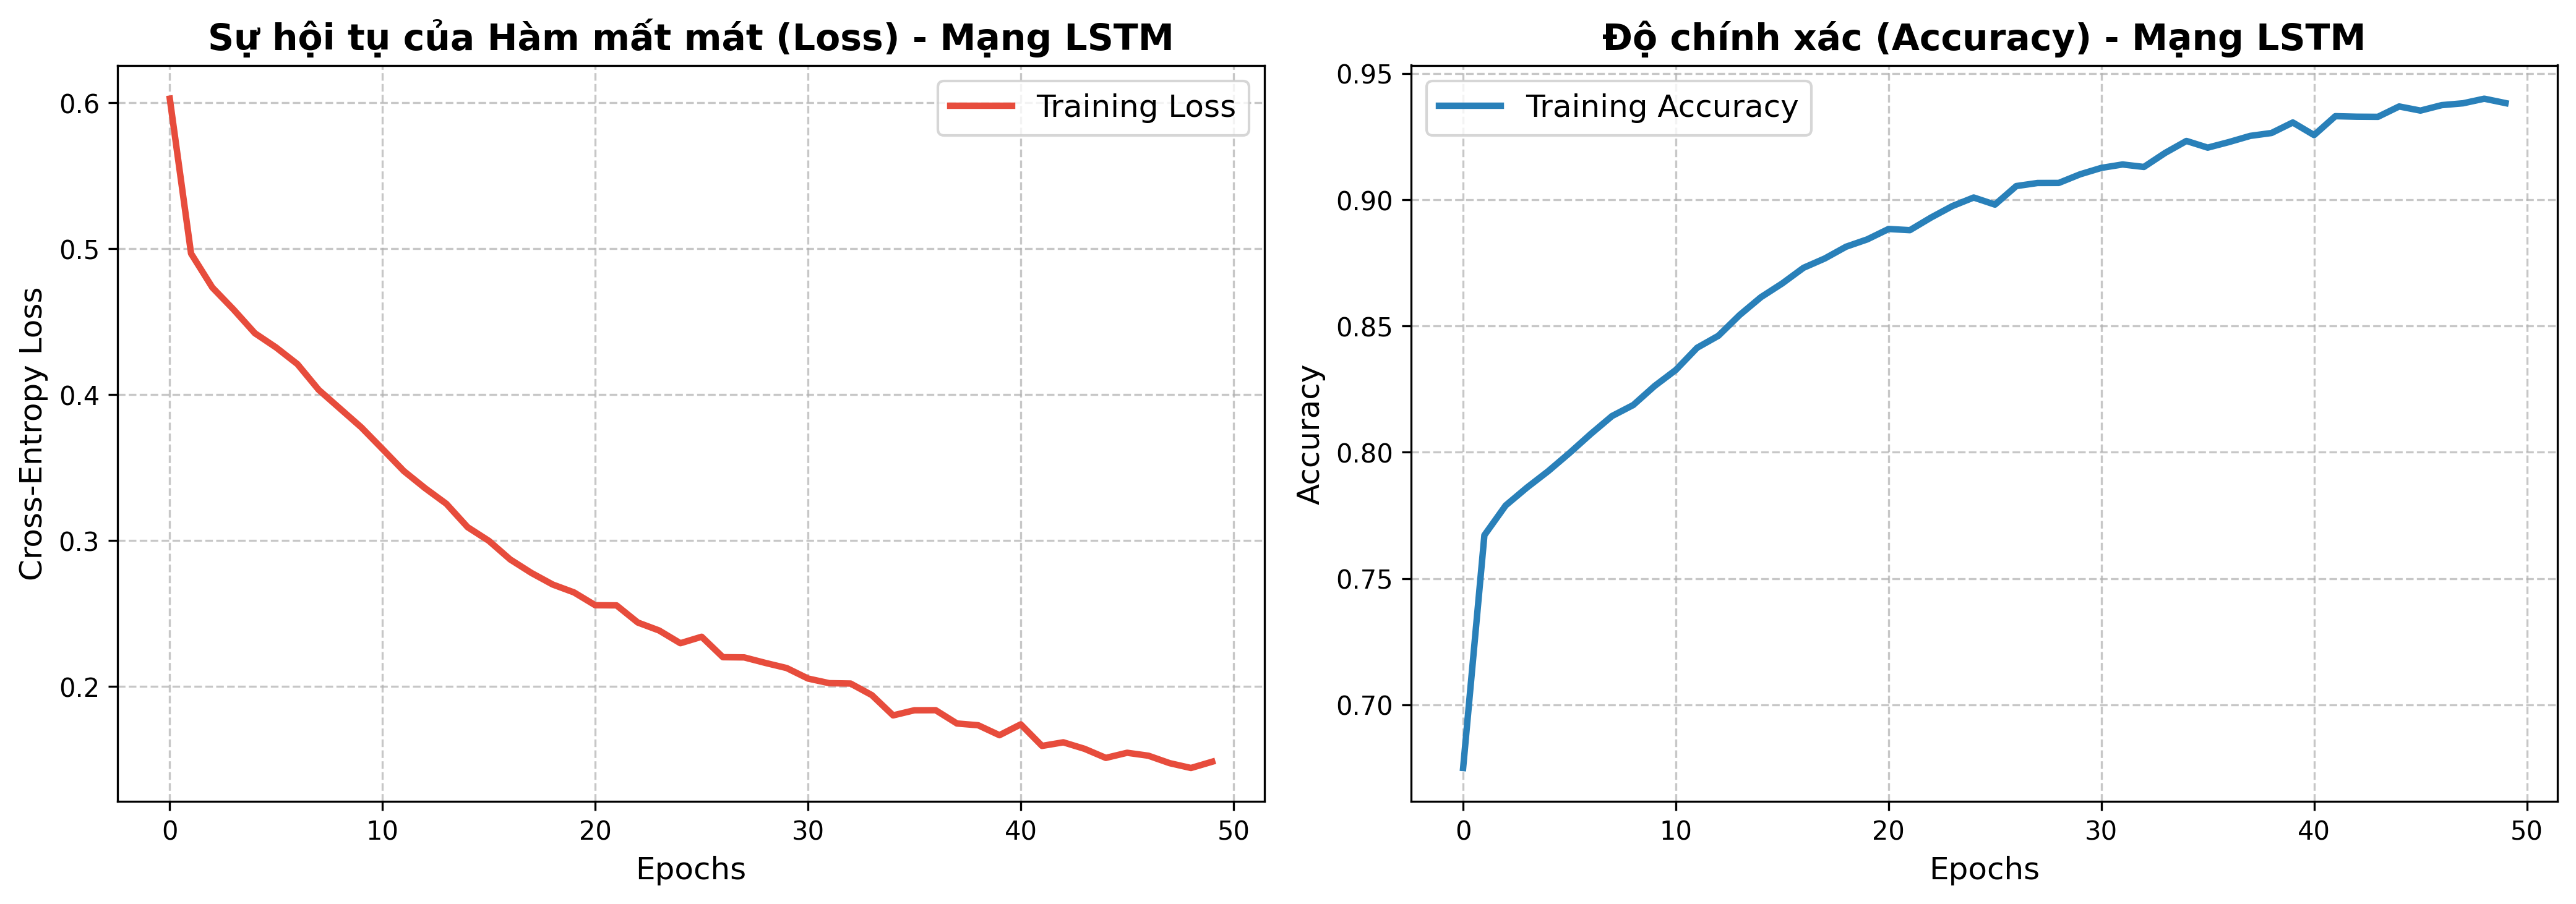
\includegraphics[width=0.9\textwidth]{images/lstm_training_results.png}
    \caption{Biểu đồ Hàm mất mát và Độ chính xác của mạng LSTM qua 50 epochs}
    \label{fig:lstm_training}
\end{figure}

Sau khi hoàn tất việc sử dụng mô hình YOLO26n để trích xuất quỹ đạo và các đặc trưng hình học, tập dữ liệu chuỗi thời gian được đưa vào mạng LSTM để thực hiện bài toán phân loại ý định nhị phân (0: Safe, 1: Cut-in). Dựa trên các chỉ số thực nghiệm thu được từ Hình \ref{fig:lstm_training}, mô hình thể hiện năng lực học tập và hội tụ ổn định qua 50 epochs:

\begin{itemize}
    \item \textbf{Sự hội tụ của hàm mất mát:} Đồ thị Training Loss cho thấy xu hướng giảm dốc đứng ngay từ những epoch đầu tiên, bắt đầu từ mức khởi điểm xấp xỉ 0.6 và hội tụ về mức khoảng 0.15 tại epoch thứ 50. Việc hàm mất mát giảm dần và ổn định ở mức thấp chứng minh mạng LSTM đã tối ưu hóa tốt việc phân biệt giữa hành vi giữ làn bình thường và ý định tạt đầu nguy hiểm dựa trên các đặc trưng vi phân bậc cao.
    
    \item \textbf{Độ chính xác:} Chỉ số Training Accuracy có sự tăng trưởng mạnh mẽ và tỷ lệ thuận với sự sụt giảm của hàm mất mát. Bắt đầu từ mức khởi điểm khoảng 67\%, độ chính xác nhanh chóng vượt ngưỡng 85\% sau 20 epoch và đạt ngưỡng ổn định xấp xỉ 94\% ở cuối quá trình huấn luyện. 
\end{itemize}

Kết quả thực nghiệm này khẳng định rằng kiến trúc kết hợp CNN-RNN hoàn toàn phù hợp để nắm bắt động học phức tạp của hành vi tạt đầu. Việc khai thác sự biến thiên của các đặc trưng logic như tỷ lệ khung hình ($AR$) và tọa độ tâm trong một cửa sổ thời gian giúp mạng LSTM nhận diện rõ ràng các mẫu hành vi phi tuyến tính của phương tiện mà các mô hình vật lý truyền thống thường bỏ lỡ. Hiệu suất 94\% đảm bảo hệ thống có khả năng đưa ra các quyết định cảnh báo sớm với độ tin cậy cao trong môi trường giao thông hỗn hợp.


% =========================================================
% 4. ĐÁNH GIÁ THỰC NGHIỆM HỆ THỐNG LAI (Hybrid Decision System)
% =========================================================
\subsection{Đánh giá thực nghiệm hệ thống lai}
Để đánh giá tính ứng dụng thực tiễn và khả năng tương tác giữa tầng trí tuệ nhân tạo (YOLO+LSTM) với tầng luật Heuristic (Zones), hệ thống được thử nghiệm trên các video giao thông hỗn hợp tại Việt Nam chưa từng xuất hiện trong tập huấn luyện. Sự đối chiếu được thực hiện giữa 3 cấu hình: (a) Toàn vẹn hệ thống YOLO+LSTM+Zones, (b) Chỉ có YOLO+LSTM, và (c) Chỉ dùng YOLO26 độc lập.

Sự phân loại ý định dựa trên ngưỡng xác suất $P_{cut} \geq 0.5$ và trạng thái xâm nhập vùng Zone.

% --- KỊCH BẢN 1 ---
\subsubsection{Kịch bản 1: Môi trường bình thường}

\begin{figure}[H]
	\centering
	\begin{subfigure}{0.32\textwidth}
		\centering
		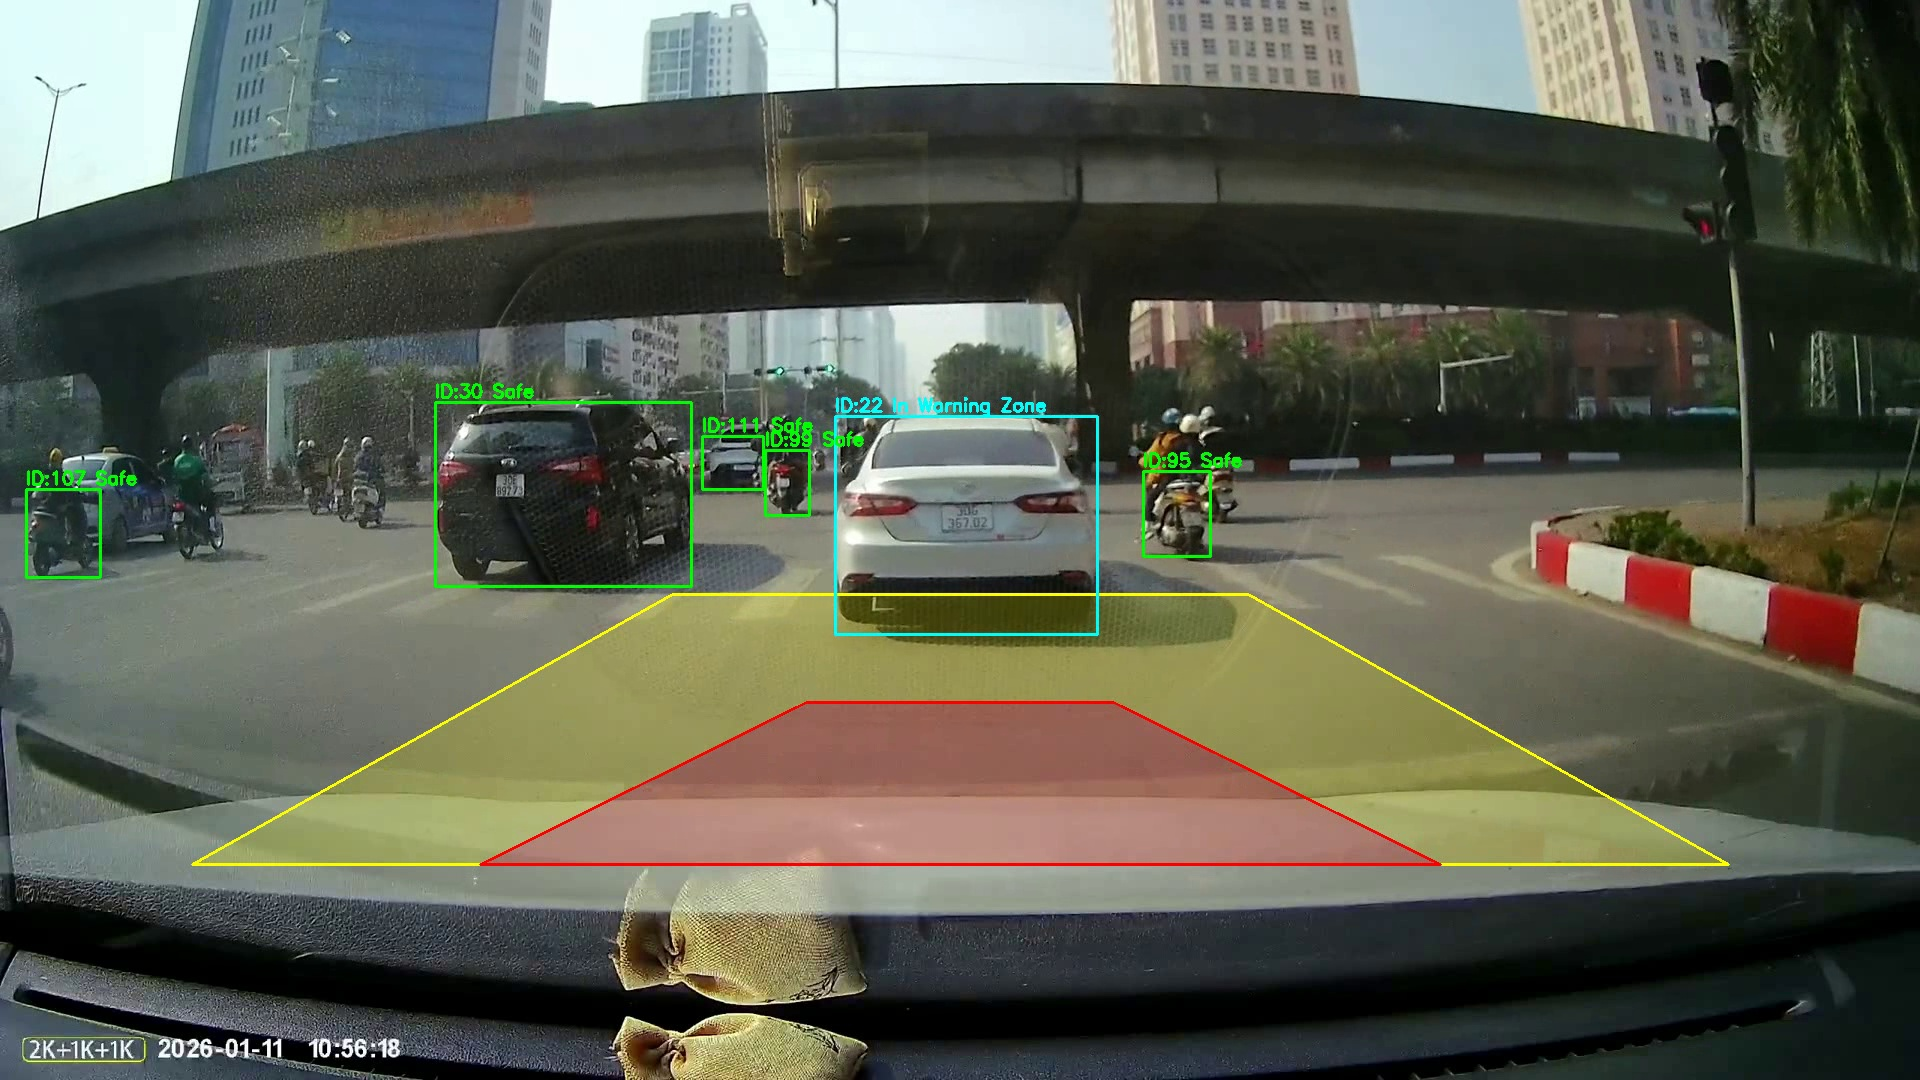
\includegraphics[width=\linewidth]{images/test/1_lstm_zone.jpg}
		\caption{YOLO26 + LSTM + Zones}
	\end{subfigure}
	\hfill
	\begin{subfigure}{0.32\textwidth}
		\centering
		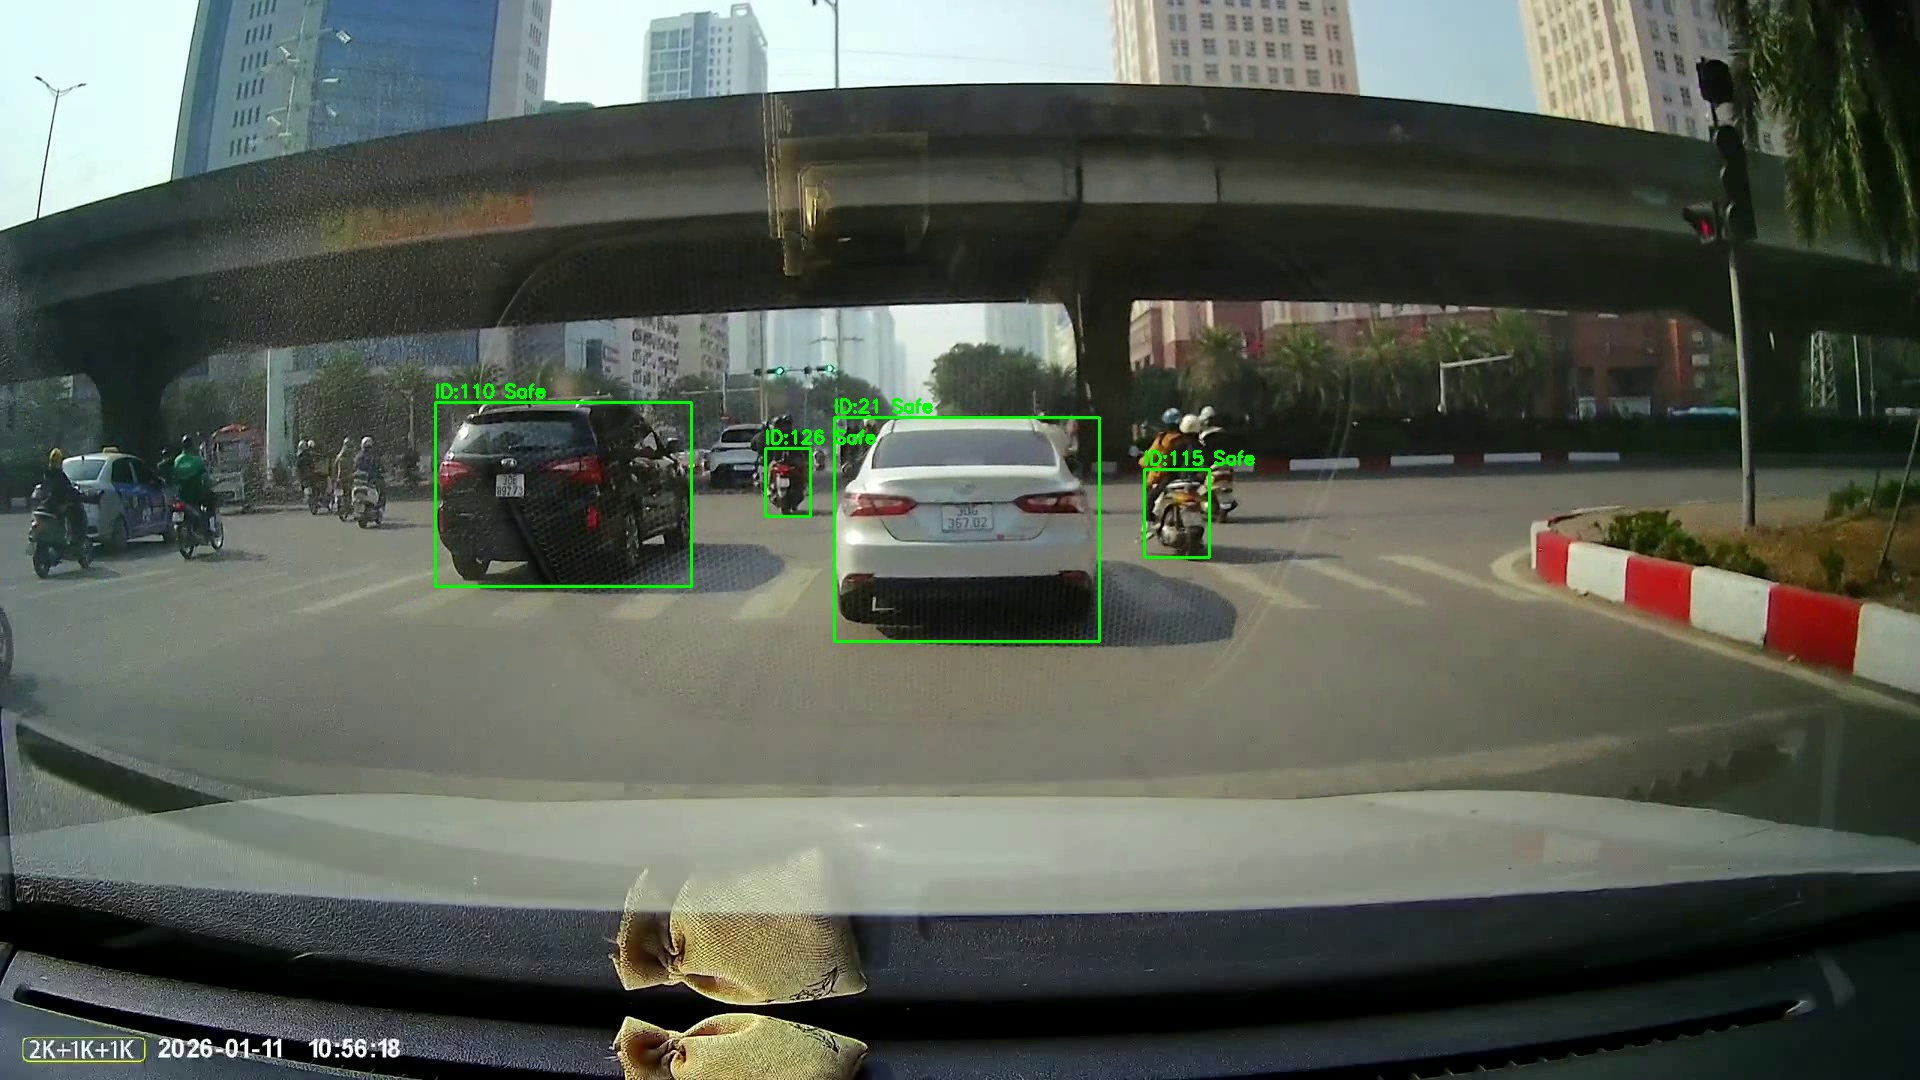
\includegraphics[width=\linewidth]{images/test/1_lstm.jpg}
		\caption{YOLO26 + LSTM}
	\end{subfigure}
	\hfill
	\begin{subfigure}{0.32\textwidth}
		\centering
		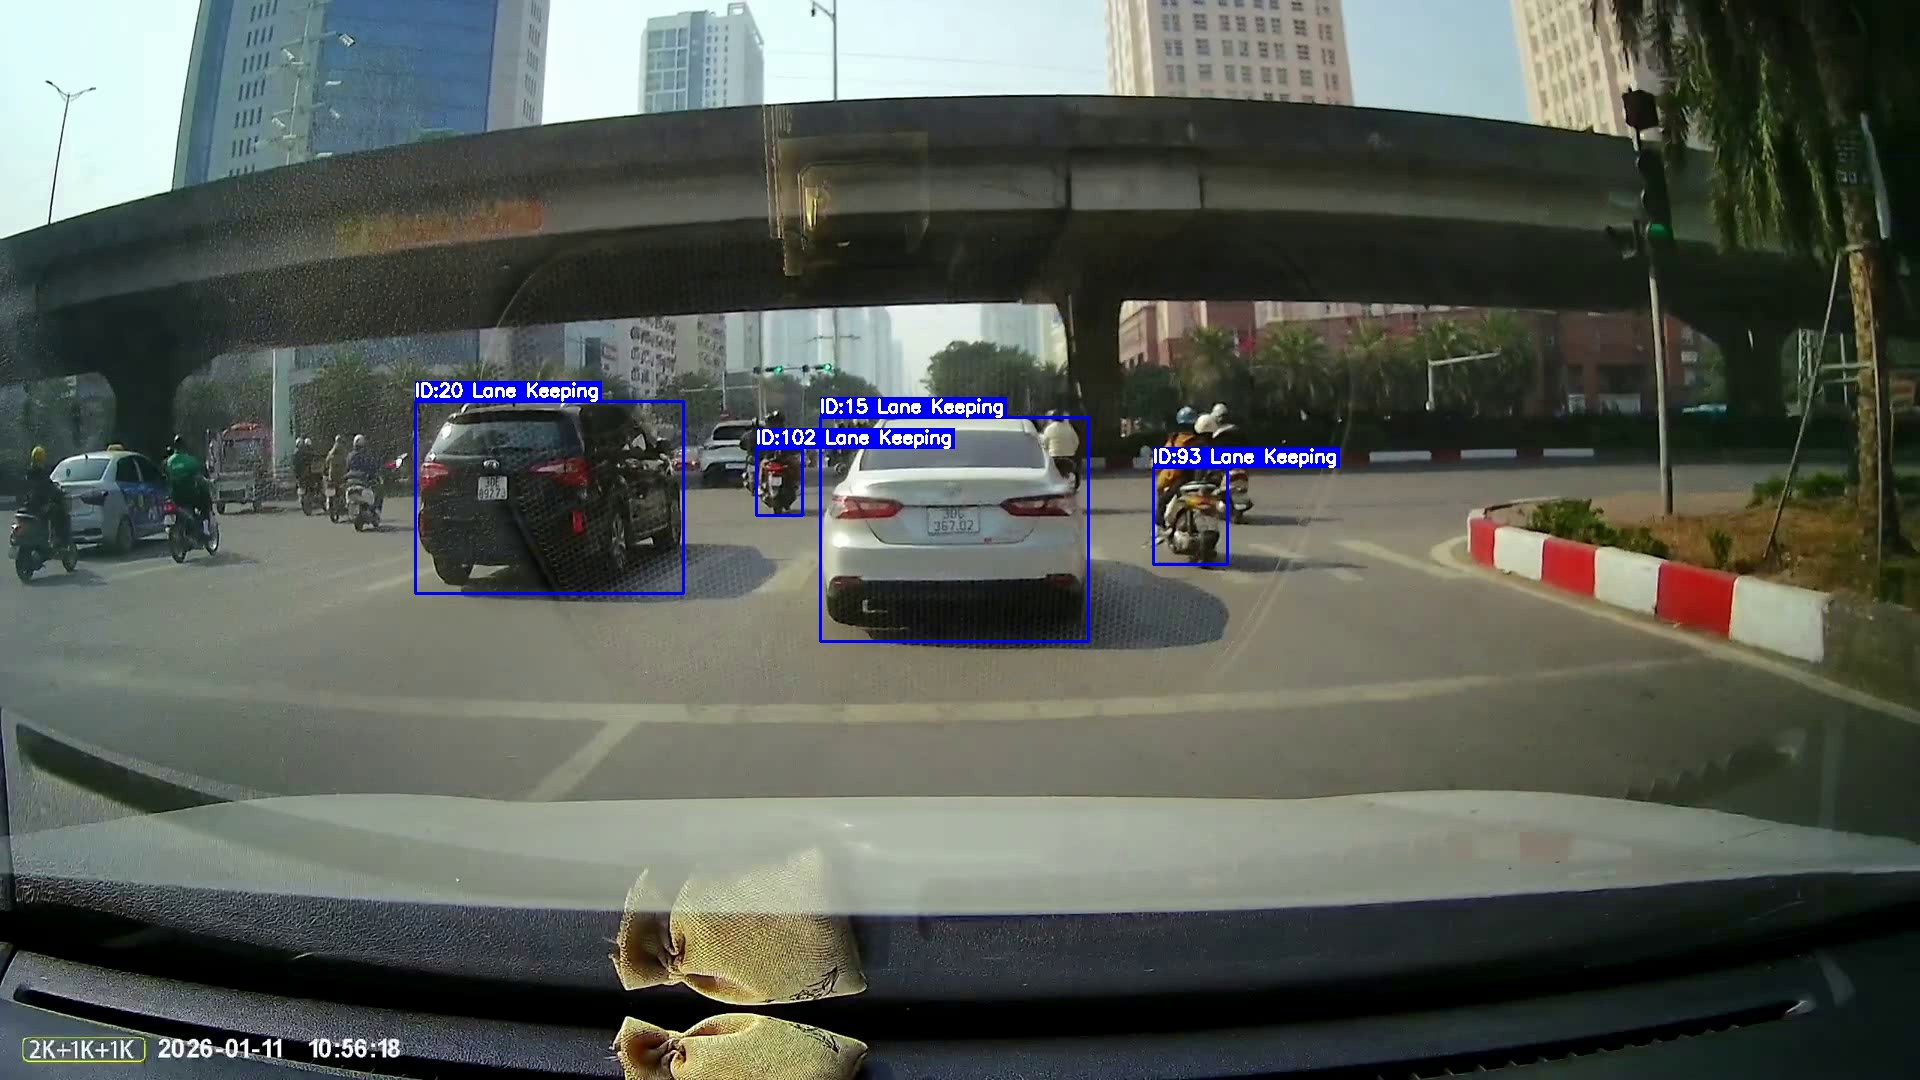
\includegraphics[width=\linewidth]{images/test/1_yolo.jpg}
		\caption{YOLO26 độc lập}
	\end{subfigure}
	\caption{Thực nghiệm trong điều kiện giao thông bình thường}
	\label{fig:normal}
\end{figure}

\textbf{Phân tích Ngữ cảnh và Kết quả (Hình \ref{fig:normal}):}
Ngữ cảnh thử nghiệm cho thấy một phương tiện đang di chuyển ổn định phía trước phương tiện máy chủ, song song với hướng di chuyển và chưa có dấu hiệu đánh lái.
\begin{itemize}
	\item \textbf{Cấu hình (c) YOLO26 độc lập}: Mô hình phát hiện chính xác đối tượng là phương tiện với độ tin cậy cao (0.82). Tuy nhiên, về mặt nhận thức, hệ thống chỉ dừng lại ở việc biết "có một phương tiện" mà không có bất kỳ thông tin nào về hành vi.
	\item \textbf{Cấu hình (b) YOLO26+LSTM}: Nhờ phân tích chuỗi tọa độ quá khứ, mạng LSTM giải mã hành vi của phương tiện là di chuyển thẳng. Xác suất tạt đầu thấp ($P_{cut} = 0.08$), nhãn hành vi hiển thị là \texttt{Lane Keeping} (Màu xanh). Hệ thống xác nhận không có rủi ro về mặt ý định.
	\item \textbf{Cấu hình (a) Hệ thống Lai toàn vẹn}: Tại đây, tầng nhận thức ý định AI và tầng không gian Heuristic Zone tương tác hoàn hảo. Mặc dù phương tiện di chuyển ổn định ($P_{cut} = 0.08$ - Xanh), việc hiển thị các vùng tĩnh \texttt{Warning Zone} (Đa giác Vàng) và \texttt{Danger Zone} (Đa giác Đỏ) đóng vai trò định khung không gian. Phương tiện nằm hoàn toàn ngoài vùng Warning, xác thực lại một lần nữa sự an toàn tuyệt đối. Cả 3 hệ thống đều không phát cảnh báo giả, đảm bảo không gây xao nhãng cho tài xế.
\end{itemize}


% --- KỊCH BẢN 2 ---
\subsubsection{Kịch bản 2: Cảnh báo sớm ý định tạt đầu}

\begin{figure}[H]
	\centering
	\begin{subfigure}{0.32\textwidth}
		\centering
		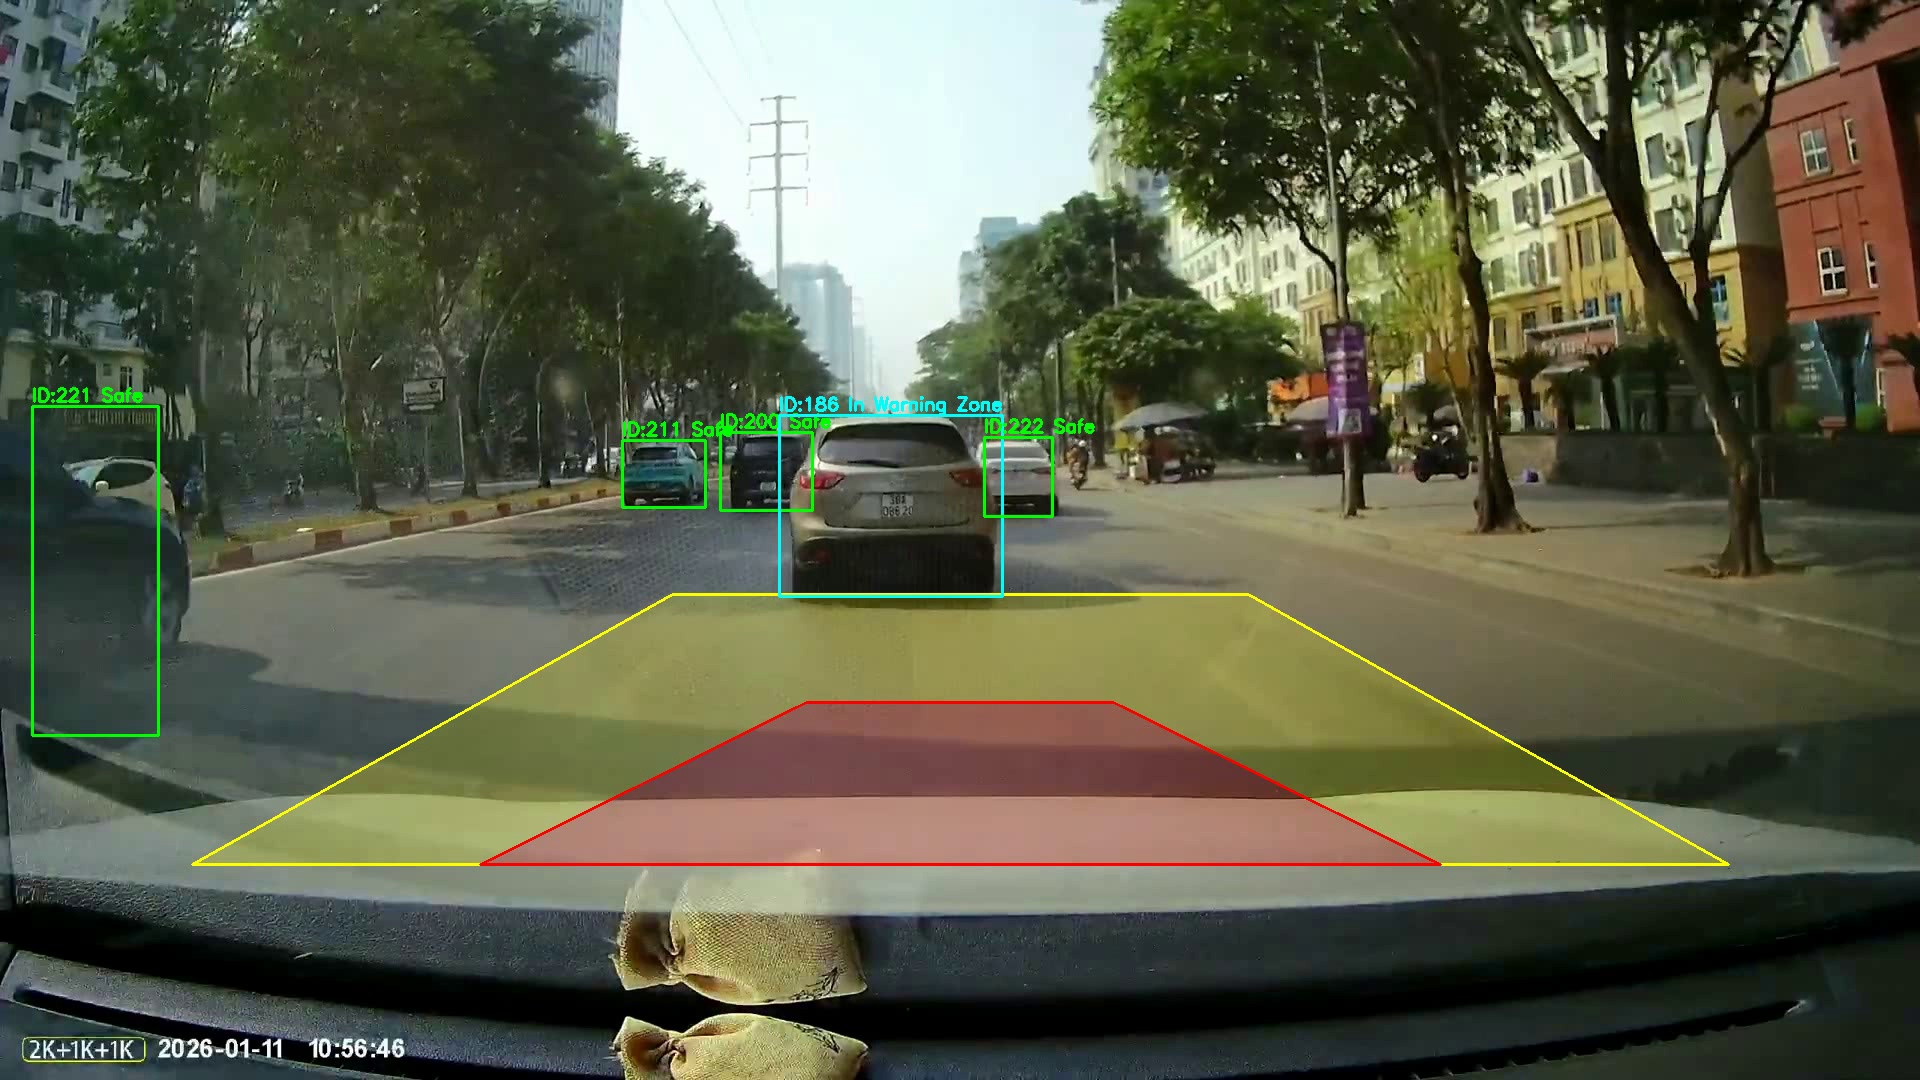
\includegraphics[width=\linewidth]{images/test/2_lstm_zone.jpg}
		\caption{YOLO26 + LSTM + Zones}
	\end{subfigure}
	\hfill
	\begin{subfigure}{0.32\textwidth}
		\centering
		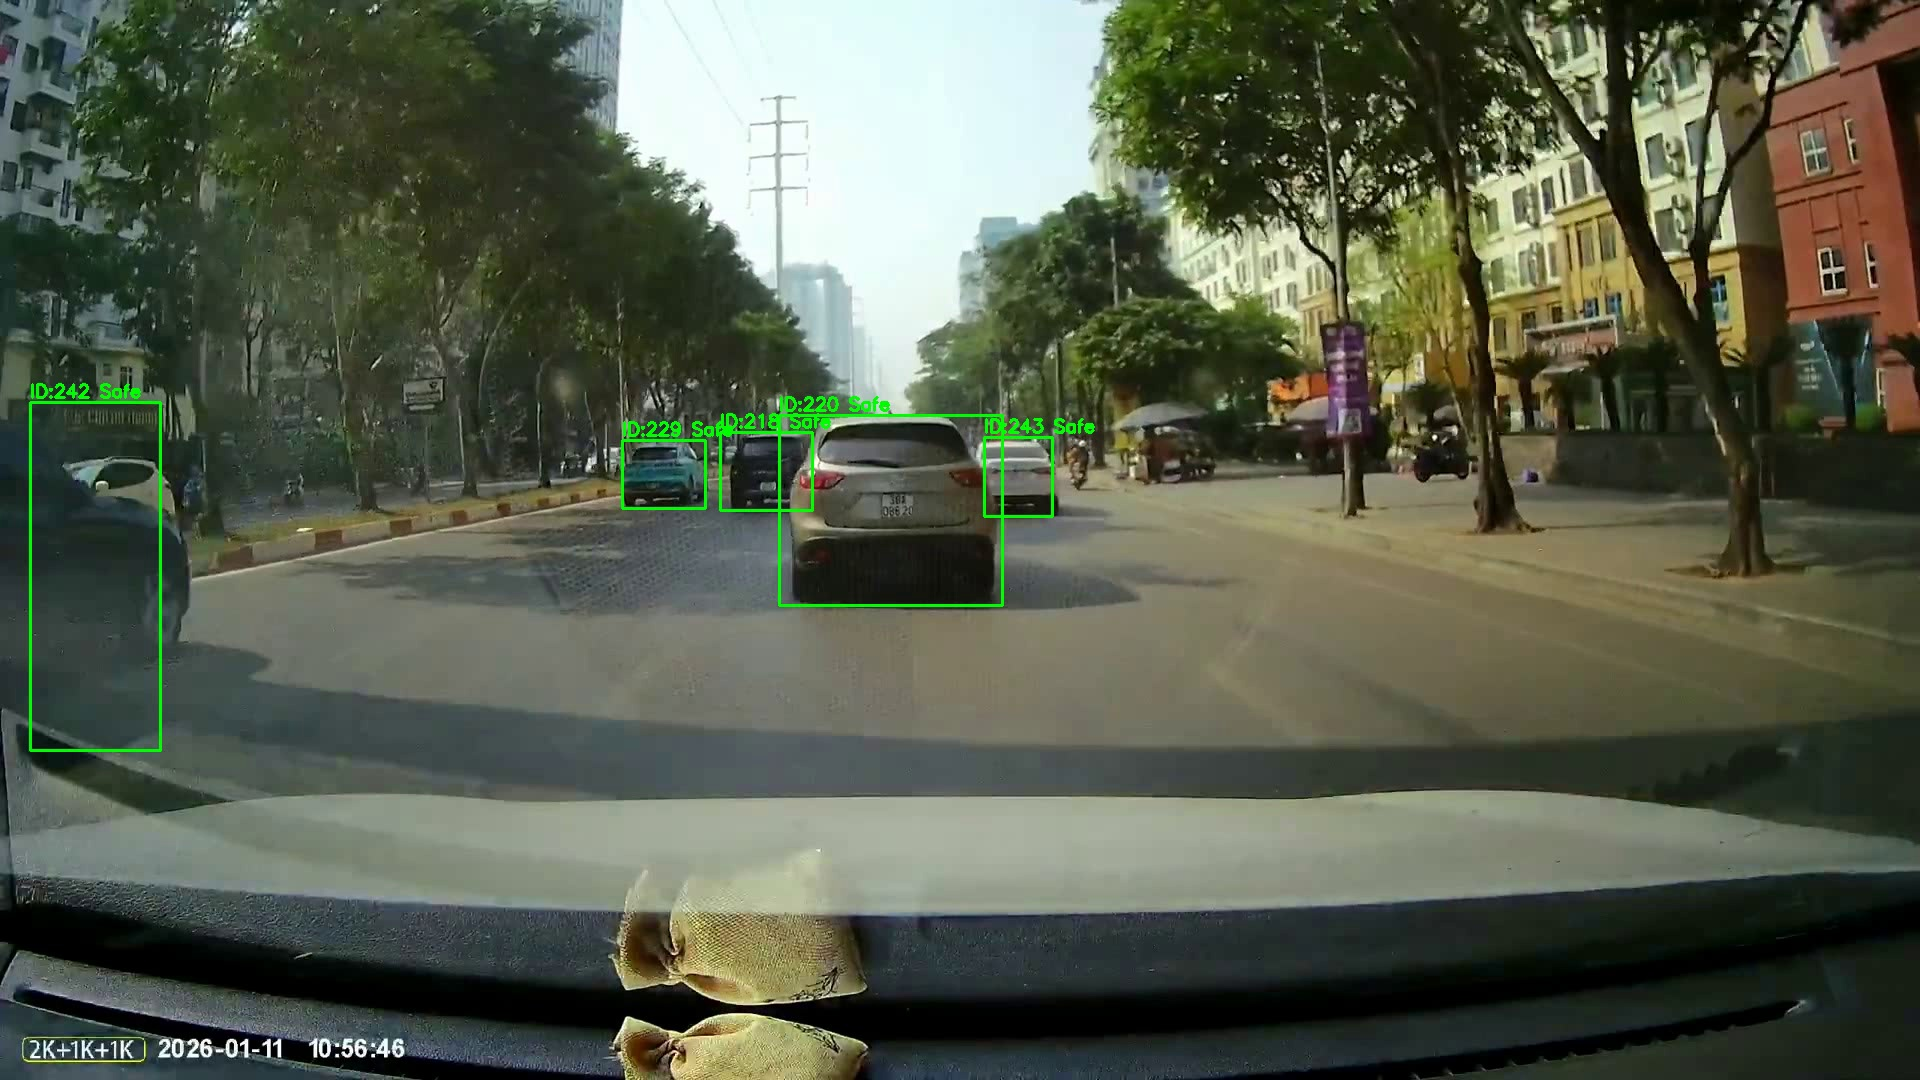
\includegraphics[width=\linewidth]{images/test/2_lstm.jpg}
		\caption{YOLO26 + LSTM}
	\end{subfigure}
	\hfill
	\begin{subfigure}{0.32\textwidth}
		\centering
		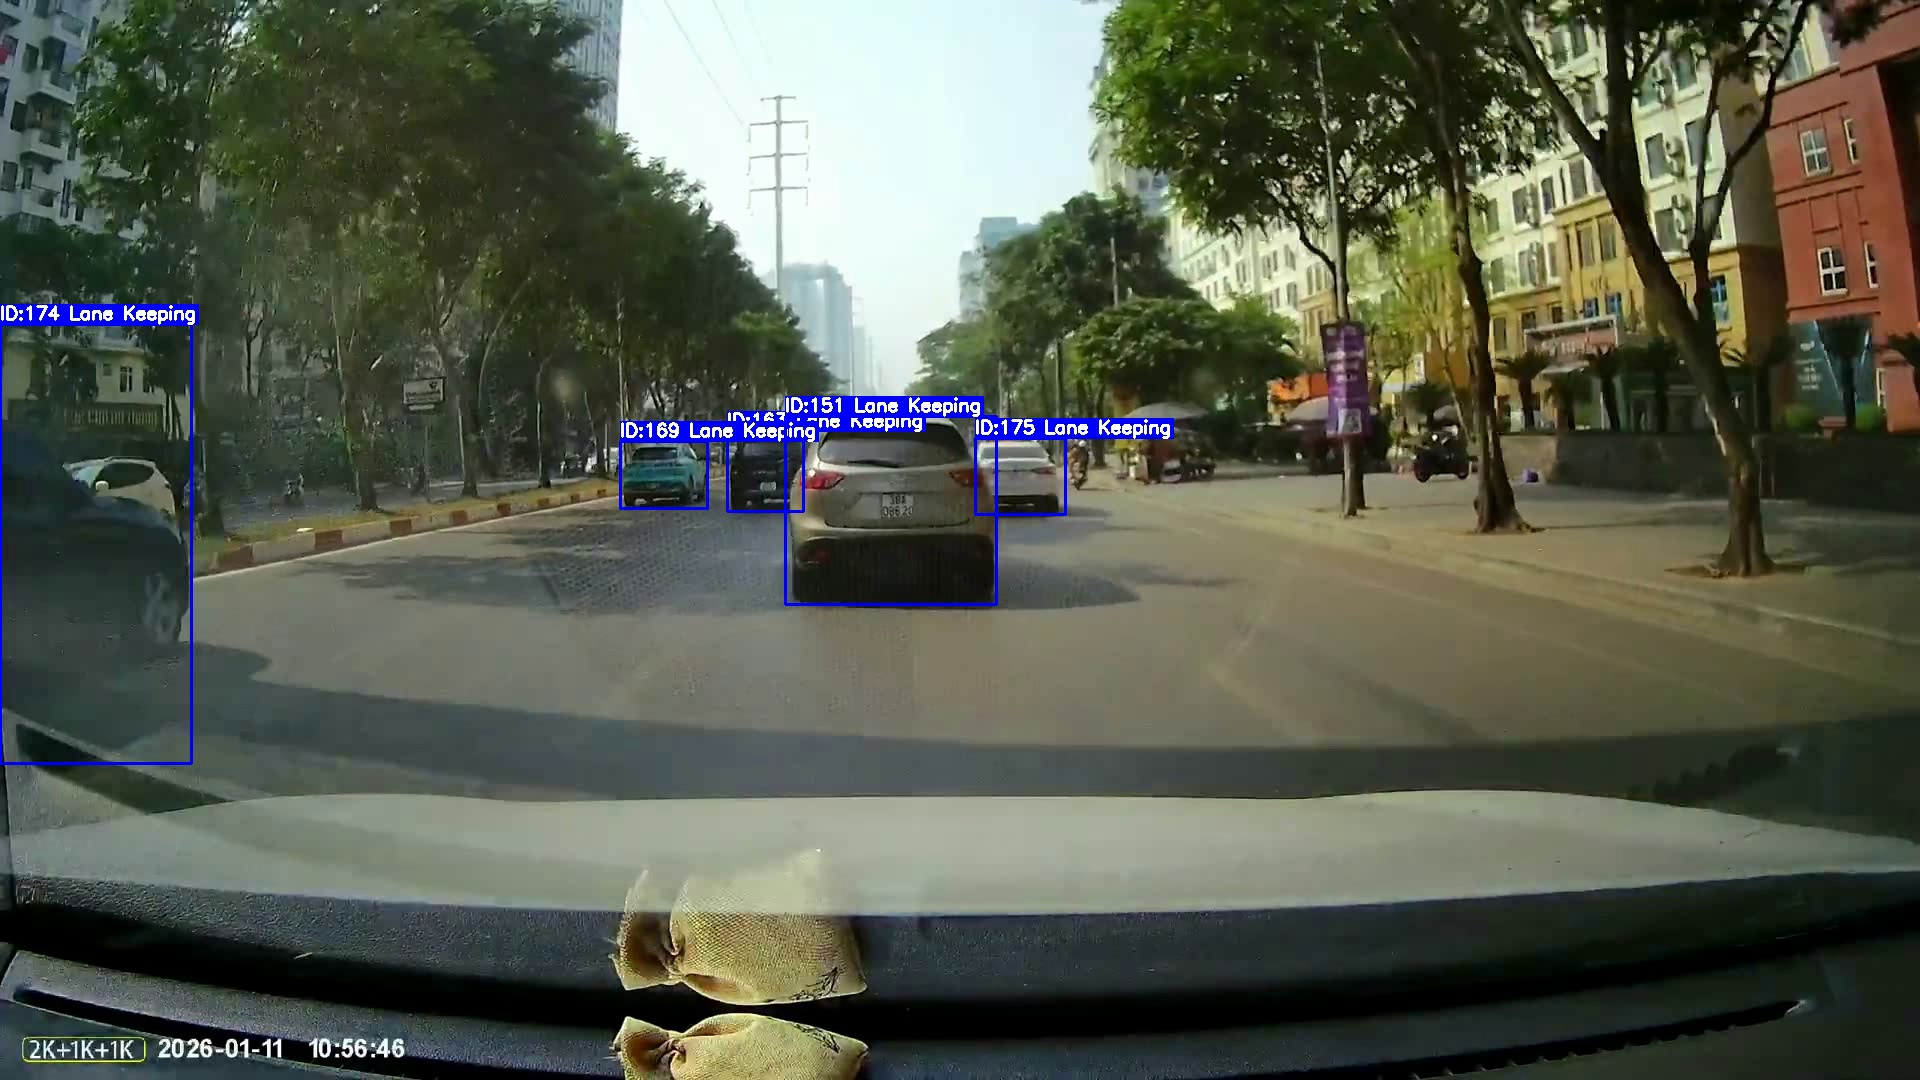
\includegraphics[width=\linewidth]{images/test/2_yolo.jpg}
		\caption{YOLO26 độc lập}
	\end{subfigure}
	\caption{Thực nghiệm năng lực cảnh báo sớm ý định tạt đầu}
	\label{fig:warning}
\end{figure}

\textbf{Phân tích Ngữ cảnh và Kết quả (Hình \ref{fig:warning}):}
Đây là kịch bản chứng minh sức mạnh của mạng LSTM. Phương tiện ở khoảng cách xa bất ngờ thực hiện động tác đánh lái, nghiêng xe để bắt đầu chuyển làn cắt ngang mui xe ô tô.
\begin{itemize}
	\item \textbf{Cấu hình (c) YOLO26 độc lập}: Thể hiện hạn chế cốt lõi của các phương pháp thuần AI tĩnh. Tại khung hình này, đối tượng chỉ là một phương tiện đang di chuyển chéo. Mô hình báo phương tiện (0.73) và hoàn toàn "im lặng" về mặt rủi ro vì nó không có nhận thức về thời gian.
	\item \textbf{Cấu hình (b) YOLO26+LSTM}: Nhờ cơ chế Window Buffer ($N=10$) và kỹ thuật lấy mẫu thưa ($S=3$), LSTM nắm bắt được sự thay đổi đột ngột của gia tốc ngang và tỷ lệ Aspect Ratio $\Delta AR$. Ngay lập tức, xác suất tạt đầu vọt lên mức rất cao ($P_{cut} = 0.96 \geq 0.5$). Hệ thống lai chuyển trạng thái cảnh báo sang mức \texttt{Cut-in Intent} (Màu Vàng).
	\item \textbf{Cấu hình (a) hệ thống lai toàn vẹn}: Điểm quan trọng nhất cần lưu ý tại Hình \ref{fig:warning}(a) là: mặc dù cảnh báo \texttt{Cut-in Intent} (Vàng) đã được kích hoạt dựa trên dự đoán AI, nhưng về mặt hình học, \textbf{đáy của Bounding Box phương tiện vẫn còn nằm ngoài đa giác Warning Zone} (chỉ nằm trên đường biên). Điều này chứng minh mạng LSTM đã cung cấp năng lực "nhìn trước" rủi ro khoảng 0.5 đến 1.0 giây so với bất kỳ hệ thống luật cứng nào chỉ dựa trên sự xâm nhập vùng không gian. AI đã giúp hệ thống phản ứng chủ động.
\end{itemize}


% --- KỊCH BẢN 3 ---
\subsubsection{Kịch bản 3: Xâm nhập vùng nguy hiểm cận chiến}

\begin{figure}[H]
	\centering
	\begin{subfigure}{0.32\textwidth}
		\centering
		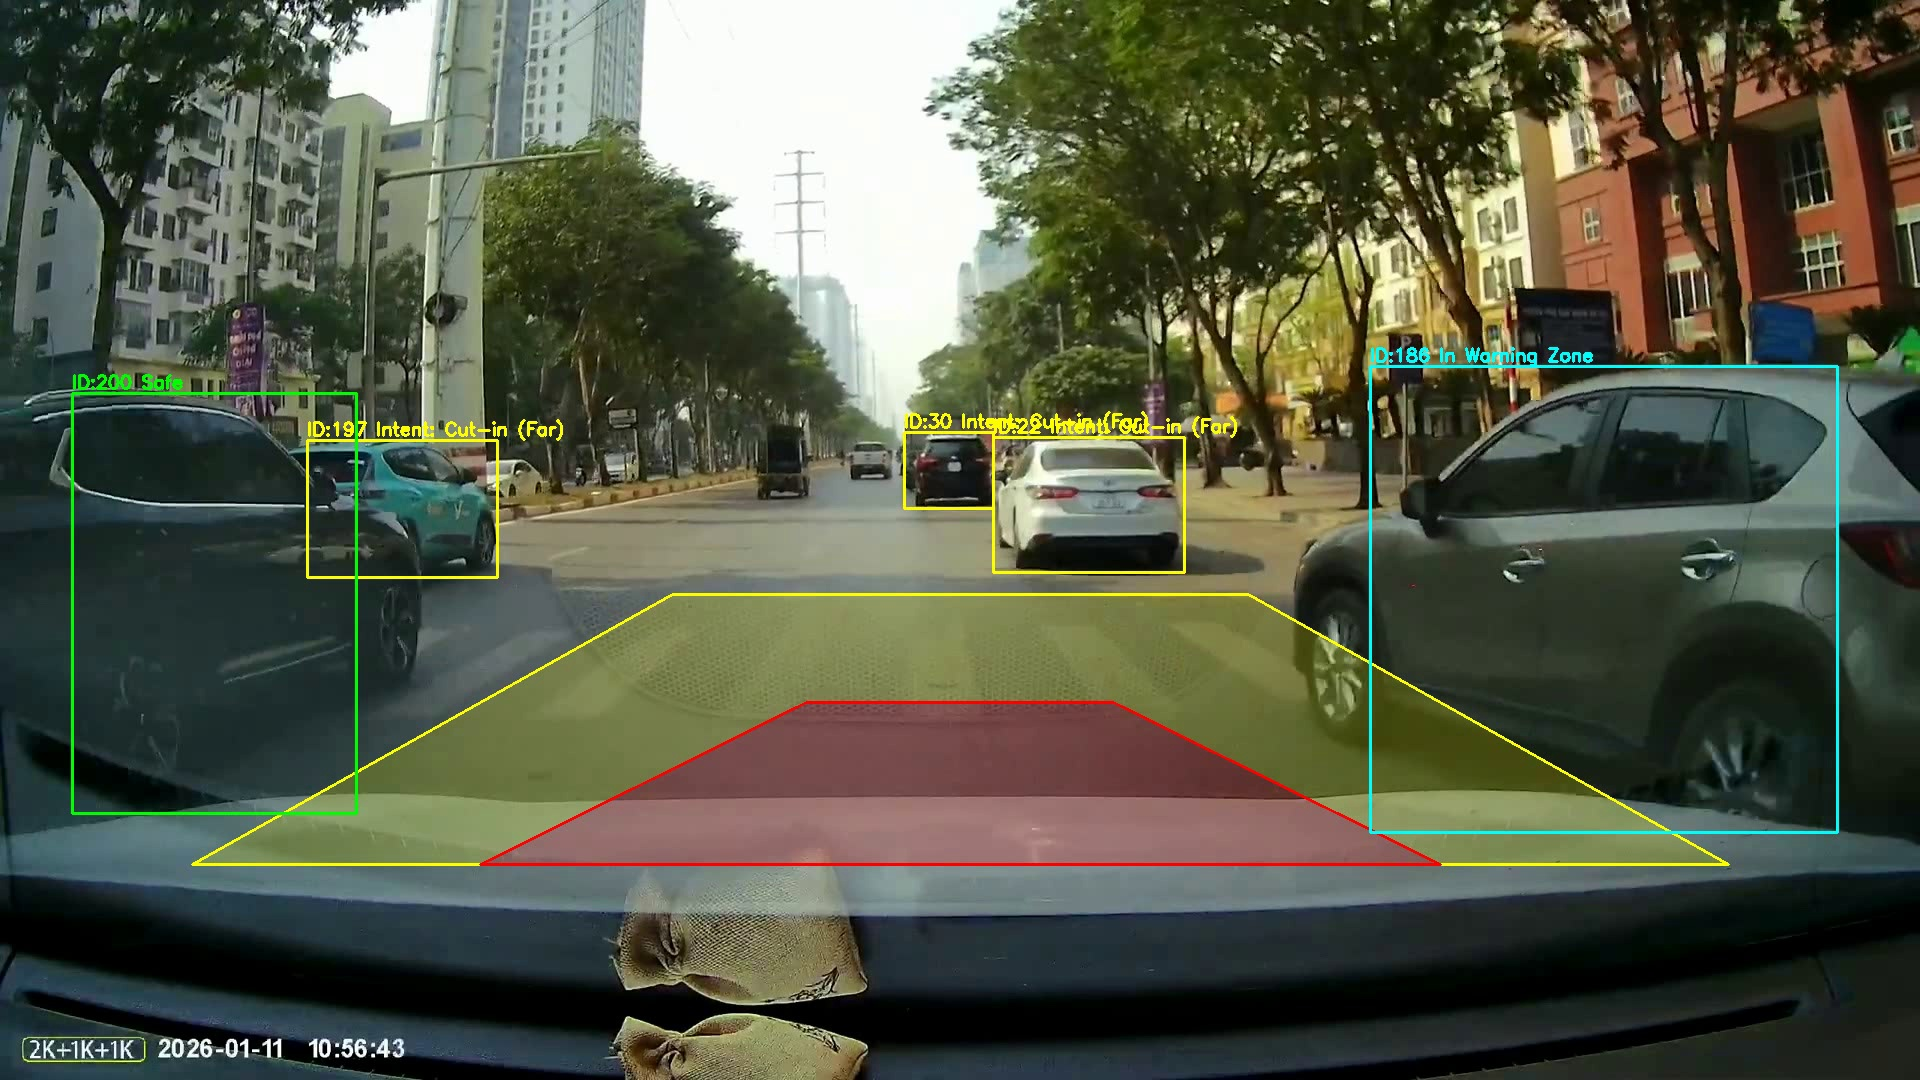
\includegraphics[width=\linewidth]{images/test/3_lstm_zone.jpg}
		\caption{YOLO26 + LSTM + Zones}
	\end{subfigure}
	\hfill
	\begin{subfigure}{0.32\textwidth}
		\centering
		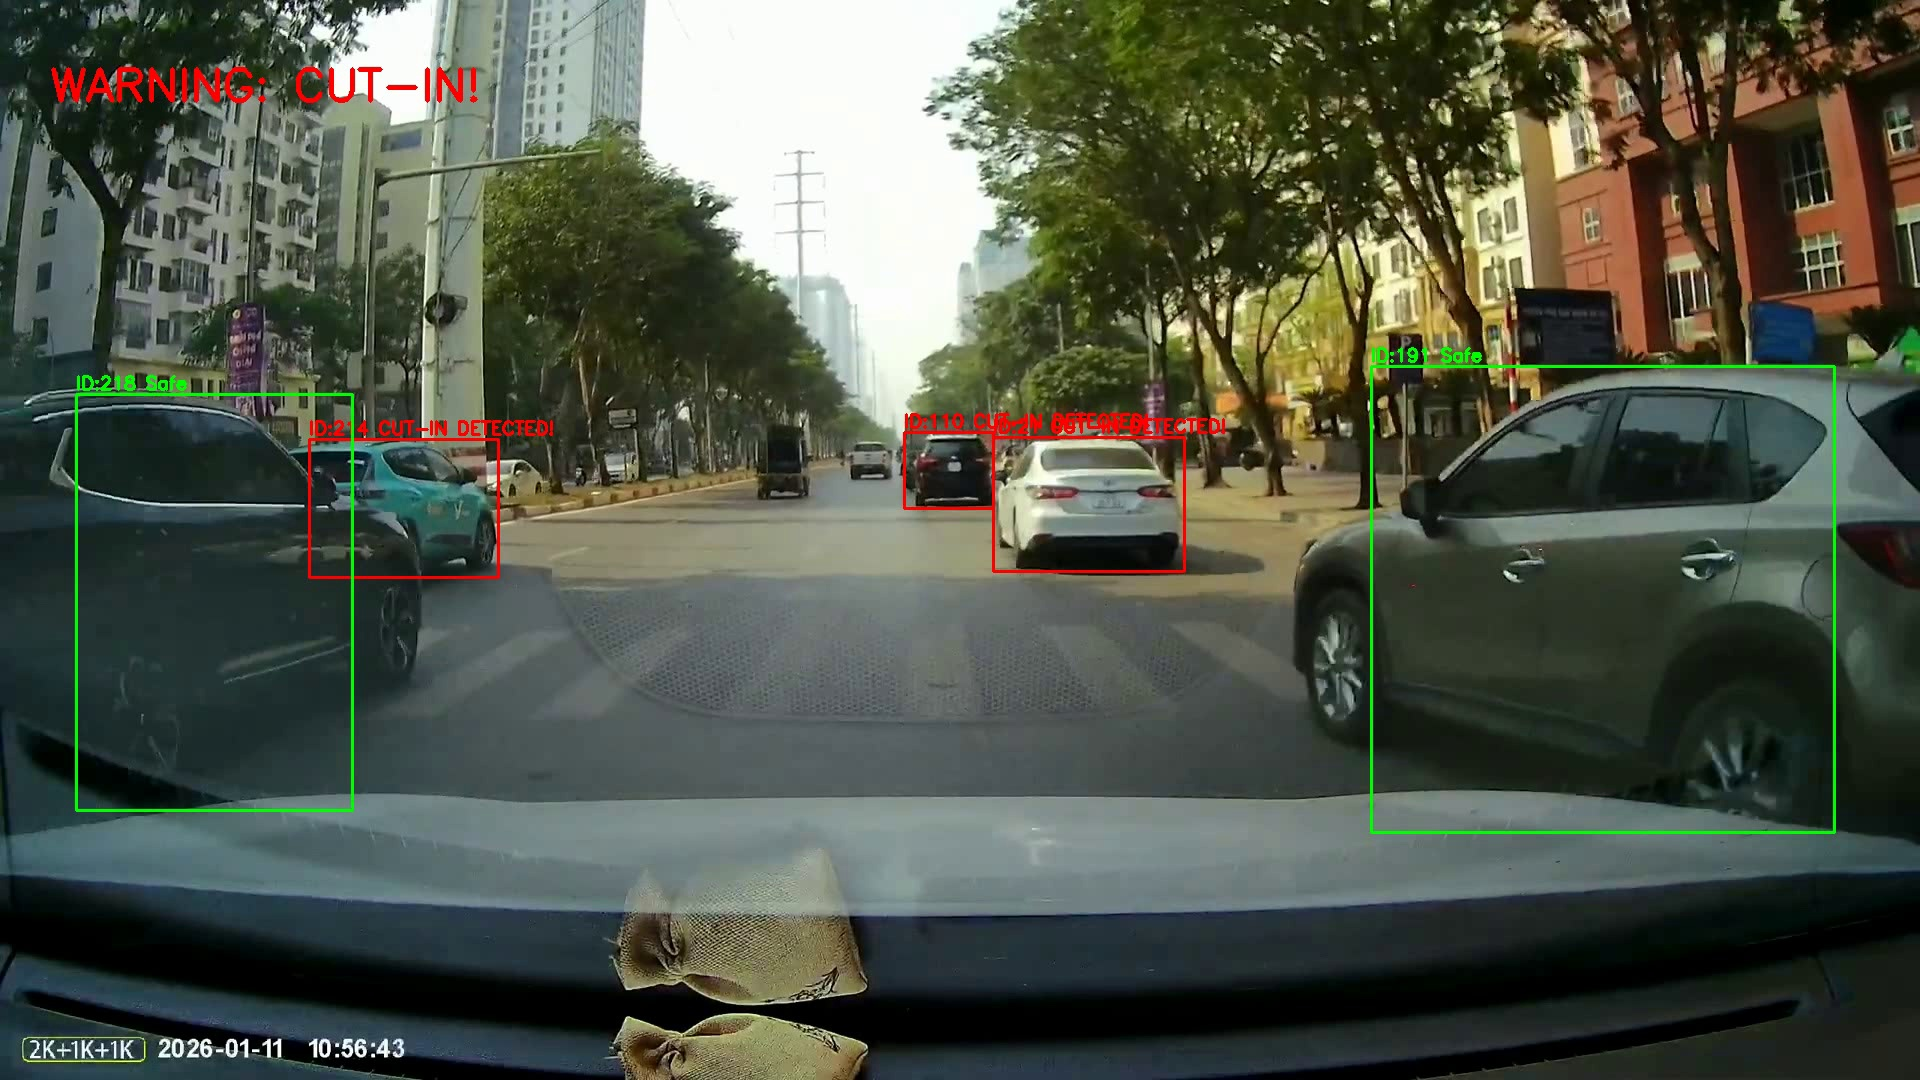
\includegraphics[width=\linewidth]{images/test/3_lstm.jpg}
		\caption{YOLO26 + LSTM}
	\end{subfigure}
	\hfill
	\begin{subfigure}{0.32\textwidth}
		\centering
		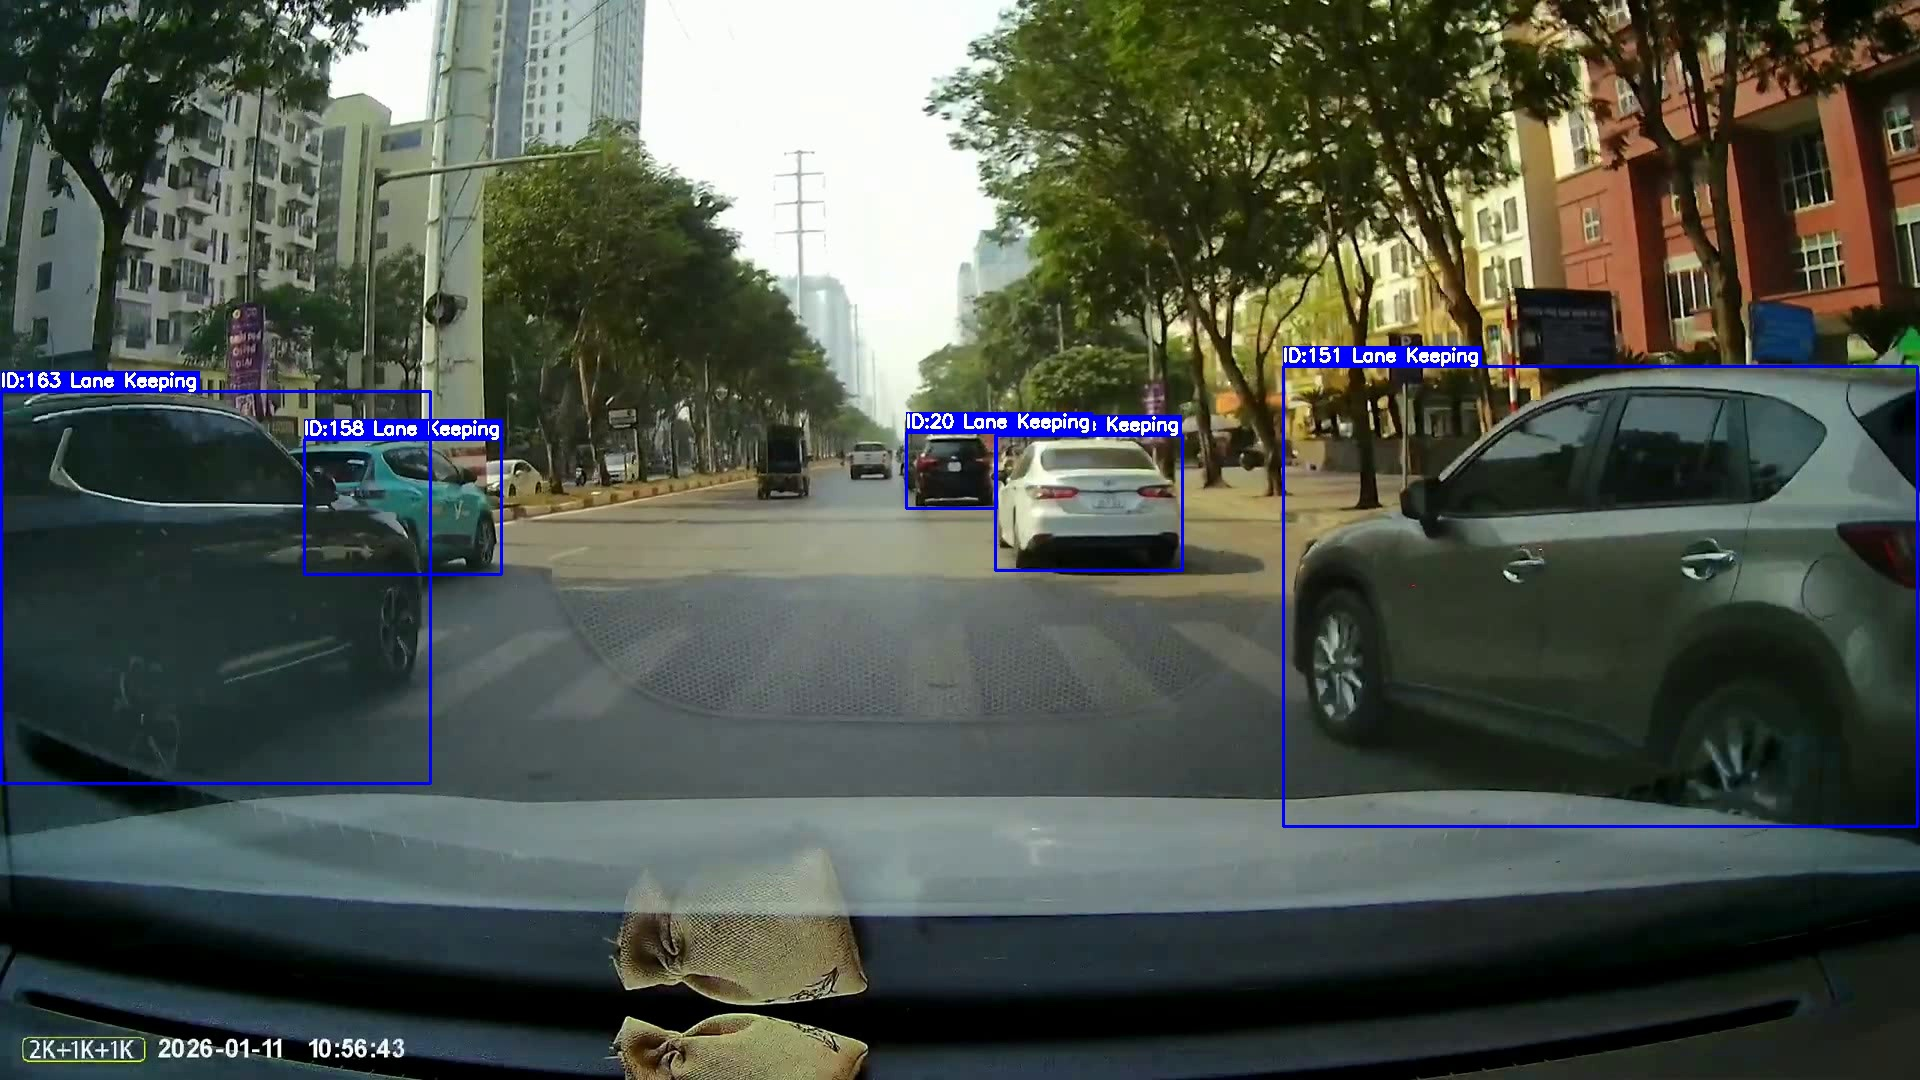
\includegraphics[width=\linewidth]{images/test/3_yolo.jpg}
		\caption{YOLO26 độc lập}
	\end{subfigure}
	\caption{Thực nghiệm khi phương tiện tạt đầu vào vùng nguy hiểm}
	\label{fig:cutin}
\end{figure}

\textbf{Phân tích Ngữ cảnh và Kết quả (Hình \ref{fig:cutin}):}
Ngữ cảnh giả lập tình huống nguy hiểm nhất: phương tiện tạt đầu ngoặt nghèo ở cự ly cực ngắn, xâm nhập sâu vào không gian ngay trước mũi xe ô tô.
\begin{itemize}
	\item \textbf{Cấu hình (c) YOLO26 độc lập}: Tiếp tục thể hiện sự "vô tri" trước rủi ro. Mô hình chỉ phát hiện phương tiện (0.81). Tài xế không nhận được bất kỳ thông tin đo lường rủi ro cận chiến nào.
	\item \textbf{Cấu hình (b) YOLO26+LSTM}: Nhận diện ý định chính xác. Quỹ đạo quá khứ confirms hành vi tạt đầu, LSTM báo $P_{cut} = 1.00$ (Màu Vàng - Intent). Tuy nhiên, về mặt ra quyết định an toàn, chỉ có thông tin $P_{cut} = 1.00$ là chưa đủ. Nếu chỉ dựa hoàn toàn vào AI, trong một mili-giây nhiễu ảnh nào đó, AI có thể tuột $P_{cut}$ xuống 0.49 và hệ thống sẽ tắt cảnh báo ngay khi phương tiện đang nằm ngay trước mui xe.
	\item \textbf{Cấu hình (a) Hệ thống Lai toàn vẹn}: Giải quyết triệt để rủi ro Black-box của AI. Hệ thống logic cảnh báo thực hiện kiểm tra chéo: LSTM báo tạt đầu ($P_{cut} = 1.00$) kết hợp với tầng luật Heuristic kiểm tra thấy đáy Bounding Box đã xâm nhập hoàn toàn vào vùng Red Danger Zone. Ngay lập tức, hệ thống kích hoạt luật cứng Fail-safe, override toàn bộ trạng thái khác, chuyển nhãn cảnh báo sang mức cao nhất: \texttt{DANGER! BRAKE} (Màu Đỏ nhấp nháy). Việc hiển thị đa giác đỏ (Zones) không chỉ xác thực cảnh báo AI mà còn định lượng chính xác được cự ly vật lý từ mũi xe ô tô đến vật cản, tạo cơ sở sống còn cho các hệ thống Phanh khẩn cấp tự động (AEB) hoạt động.
\end{itemize}

\section{Thảo luận về tính bền vững và khả năng thích nghi}
\subsection{Hiệu suất trong các điều kiện ánh sáng biến đổi}
Một hệ thống ADAS hiệu quả phải có khả năng vận hành ổn định trong nhiều điều kiện môi trường khác nhau. Nghiên cứu thực hiện kiểm tra chéo mô hình YOLO26n trên hai tập dữ liệu con: Ban ngày (Ánh sáng thuận lợi) và Chói sáng/Bóng râm (Điều kiện khó).

\begin{itemize}
    \item \textbf{Điều kiện ban ngày:} Mô hình đạt mAP@50 ổn định ở mức 0.96. Bounding Box bao quanh vật thể có độ rung lắc (jitter) cực thấp, giúp chuỗi tọa độ đầu vào cho LSTM rất sạch.
    \item \textbf{Điều kiện chói sáng/Bóng râm:} Độ chính xác giảm nhẹ xuống 0.92. Lỗi thường gặp là Bounding Box bị co lại hoặc dãn ra đột ngột do hiện tượng tán xạ ánh sáng tại biên vật thể. Tuy nhiên, nhờ lớp LSTM có khả năng học quy luật thời gian, những sai số hình học tức thời này đã được lọc bỏ, giúp tín hiệu ý định \texttt{cut\_in} vẫn duy trì được độ tin cậy > 90\%.
\end{itemize}

\subsection{Sự đánh đổi giữa độ nhạy và cảnh báo giả}
Trong bài toán tạt đầu nguy hiểm, việc bỏ sót (\textit{False Negative}) mang lại rủi ro cao hơn nhiều so với cảnh báo nhầm (\textit{False Positive}). 
Hệ thống lai đã giải quyết sự đánh đổi này bằng cách:
\begin{enumerate}
    \item Thiết lập ngưỡng xác suất LSTM thấp ($P_{cut} \geq 0.5$) để tăng tối đa độ nhạy đối với các hành vi nghiêng xe sớm.
    \item Sử dụng các vùng \texttt{Warning Zone} để kìm hãm các cảnh báo giả ở cự ly xa (nơi xe máy có thể nghiêng người nhưng chưa đe dọa trực tiếp đến an toàn của xe máy chủ).
    \item Chỉ kích hoạt cảnh báo cưỡng bức (Level 4) khi có sự xác nhận đồng thời từ cả AI (Ý định) và Quy tắc hình học (Vị trí vật lý).
\end{enumerate}
Cơ chế này giúp hệ thống đạt được sự cân bằng: vừa "nhìn xa trông rộng" nhờ AI, vừa "vững chãi, an toàn" nhờ luật cứng.